\documentclass[11pt,a4paper]{article}
\usepackage[margin=2.4cm]{geometry}
%\usepackage[T1]{fontenc}
%\usepackage{lmodern}
\usepackage{amsmath,amssymb,mathtools,bm}
\usepackage{booktabs,tabularx,array}
\usepackage{enumitem}
\usepackage{tikz}
\usetikzlibrary{positioning,fit,arrows.meta,backgrounds}
\usepackage[most]{tcolorbox}
\usepackage[hidelinks]{hyperref}
\usepackage{xcolor}
\usepackage{url}
\urlstyle{tt}
\makeatletter\g@addto@macro{\UrlBreaks}{\do\_\do\.}\makeatother
\setlength{\parindent}{0pt}
\setlength{\parskip}{6pt}
\setlist{itemsep=2pt,topsep=3pt}

\definecolor{exbg}{RGB}{238,244,252}
\definecolor{exfr}{RGB}{40,90,160}
\definecolor{kbg}{RGB}{245,245,240}
\definecolor{kfr}{RGB}{120,120,100}
\definecolor{wbg}{RGB}{253,243,235}
\definecolor{wfr}{RGB}{190,100,40}

\newtcolorbox{exercise}[1]{colback=exbg,colframe=exfr,fonttitle=\bfseries,title={#1},breakable}
\newtcolorbox{keybox}[1]{colback=kbg,colframe=kfr,fonttitle=\bfseries,title={#1},breakable}
\newtcolorbox{warnbox}[1]{colback=wbg,colframe=wfr,fonttitle=\bfseries,title={#1},breakable}

\newcommand{\N}{\mathcal{N}}
\newcommand{\F}{\mathcal{F}}
\newcommand{\R}{\mathbb{R}}
\newcommand{\E}{\mathbb{E}}
\newcommand{\T}{^{\top}}
\DeclareMathOperator{\Var}{Var}
\DeclareMathOperator{\Cov}{Cov}
\DeclareMathOperator{\diag}{diag}
\DeclareMathOperator{\softmax}{softmax}
\DeclareMathOperator*{\argmax}{arg\,max}

\tikzset{
  lat/.style={circle,draw,minimum size=11mm,inner sep=1pt},
  obs/.style={circle,draw,fill=gray!25,minimum size=11mm,inner sep=1pt},
  par/.style={rectangle,draw,fill=black,minimum size=1.6mm,inner sep=0pt},
  edge/.style={-{Latex[length=2.2mm]},thick},
  plate/.style={draw,rounded corners,inner sep=6pt}
}

\title{Formulating a Mixture of Experts with a Hidden Markov Gate\\[4pt]
\large From Bishop's mixture of experts to a regime-gated cross-sectional return model}
\author{Course notes for Tom Kores Lesjak\\ \small Master Thesis, SAIF / SJTU}
\date{Compiled 1 October 2026; revised 5 October 2026}

\begin{document}
\maketitle
\tableofcontents
\newpage

\section*{How to use these notes}
\addcontentsline{toc}{section}{How to use these notes}

These notes build the thesis model one layer at a time, starting from Bishop's textbook mixture of experts and ending with the full regime-gated model. They cover the \emph{formulation} only: what the model is, which distribution it defines, what its likelihood is, and what it predicts. How we train it in the code (Adam, early stopping, walk-forward folds) comes later.

The order is deliberate.
\begin{enumerate}
  \item \textbf{Section 1} translates Bishop's notation into ours.
  \item \textbf{Section 2 is the warm-up}: a reading guide to Chamroukhi \& Nguyen (2018) and Bishop, followed by two exercises. Exercise A1 is a mixture of experts with \emph{linear-regression} experts and a softmax gate. Exercise A2 replaces the softmax gate with a hidden Markov chain. Because the experts are linear, EM has closed-form steps, so you can carry out every derivation by hand.
  \item \textbf{Sections 3 to 5} replace the linear experts with MLPs. They explain where the softmax gate comes from, why gradient training of the likelihood behaves like EM, how backpropagation works, and how the softmax gate becomes an HMM gate.
  \item \textbf{Sections 6 to 9} assemble our model: the full generative model, the likelihood, prediction and posteriors, and a checklist of assumptions and open design choices.
  \item \textbf{Appendices A and B} give the full solutions to the two exercises. \emph{Attempt the exercises first.}
  \item \textbf{Appendix D} gives the theory of the per-date and per-row likelihoods behind Q24.
\end{enumerate}

\subsection*{Notation used throughout}

\begin{center}
\renewcommand{\arraystretch}{1.25}
\begin{tabularx}{\textwidth}{@{}lX@{}}
\toprule
Symbol & Meaning \\
\midrule
$t = 1,\dots,T$ & trading day \\
$i \in \mathcal S_t$, $N_t = |\mathcal S_t|$ & stocks in the universe on day $t$ \\
$x_{i,t}\in\R^d$ & characteristics of stock $i$, known at the close of day $t$ \\
$r_{i,t+1}$ & the \textbf{target}: the \emph{market-neutral} return of stock $i$ over $(t,t+1]$, i.e.\ its return minus that day's equal-weighted cross-sectional mean (decided 2026-10-01, Q25) \\
$m_t$ & the gate's input series: the daily log return of the CRSP value-weighted S\&P 500 index (Q23) \\
$\F_t=\sigma(m_1,\dots,m_t)$ & the gate's information at the close of day $t$: the $\sigma$-algebra generated by the market series up to $t$. The family $(\F_t)_{t\ge1}$ is a filtration (Section 1.4) \\
$\mathcal G_t\supseteq\F_t$ & all information at the close of $t$: market series, characteristics and returns up to $t$ \\
$z_t\in\{1,\dots,K\}$ & market regime on day $t$ (one-hot vector $z_{tk}$) \\
$A_{jk}$, $\rho_k$ & transition probability $p(z_{t+1}{=}k\mid z_t{=}j)$ and initial probability $p(z_1{=}k)$ \\
$\eta_t(k)=\N(m_t;\nu_k,\sigma_k^2)$ & gate emission density: market series in regime $k$ \\
$\xi_{t\mid\tau}(k)$ & $p(z_t{=}k\mid m_1,\dots,m_\tau)$: filtered ($\tau=t$), predicted ($\tau=t-1$), smoothed ($\tau=T$) \\
$\pi_k(t)=\mathbb P(z_{t+1}{=}k\mid\F_t)$ & the gate: weight of expert $k$ for the day-$(t{+}1)$ return \\
$\mu_k(x)=f_0(x)+c_k(x;\psi_k)$ & mean of expert $k$: frozen base plus correction \\
$s_k$ & noise standard deviation of expert $k$ \\
$\gamma$ & responsibility: posterior probability of a regime or expert after seeing the returns \\
\bottomrule
\end{tabularx}
\end{center}

\begin{warnbox}{Notation clashes to keep in mind}
\begin{itemize}
  \item Bishop writes the \emph{target} as $t$; here $t$ is always time.
  \item \path{Model_Derivation_BaseCase.md} uses $s_t$ for the regime, $\mathbf P$ for the transition matrix, $r_t$ for the market series, $\mu_k$ for the gate mean, and $r_k$ for the expert corrections. In these notes those are $z_t$, $A$, $m_t$, $\nu_k$ and $c_k$, which frees $r$ for returns and $\mu$ for expert means.
  \item $\sigma_k$ is always the \emph{gate's} regime volatility of the market series. $s_k$ is always the \emph{expert's} noise. They measure different things (Section 3.3).
  \item Chamroukhi \& Nguyen use $\pi$ both for the HMM initial distribution and for the logistic gate. They use $\alpha_k$ for constant mixing proportions, $\tau$ for cluster posteriors, $\gamma$ for regime posteriors, and $\xi$ for pairwise posteriors.
\end{itemize}
\end{warnbox}
\newpage

\section{From Bishop's mixture of experts to our model}

\subsection{Bishop's starting point and the hidden latent variable}

Bishop (\S14.5.3) writes a mixture of experts as
\begin{equation}\label{eq:bishop-moe}
p(y\mid x) = \sum_{k=1}^{K} \pi_k(x)\, p_k(y\mid x).
\end{equation}
(Bishop writes the target as $t$; we write it as $y$.) No latent variable appears in \eqref{eq:bishop-moe}, because it has already been \emph{summed out}. Introduce a one-hot vector $z$ whose component $z_k=1$ means ``expert $k$ generated this observation''. The model then consists of two statements:
\begin{equation}
p(z_k=1\mid x)=\pi_k(x), \qquad p(y\mid x, z_k=1) = p_k(y\mid x).
\end{equation}
Using the exponent trick of Bishop (9.10)--(9.11), the joint distribution is
\begin{equation}
p(y,z\mid x) = p(z\mid x)\,p(y\mid x,z) = \prod_{k=1}^K \big[\pi_k(x)\,p_k(y\mid x)\big]^{z_k}.
\end{equation}
Because $z$ is never observed, we sum it out. Each value of $z$ switches on exactly one factor, so
\begin{equation}
p(y\mid x)=\sum_z p(y,z\mid x)=\sum_{k=1}^K \pi_k(x)\,p_k(y\mid x).
\end{equation}
The latent variable is therefore still present in \eqref{eq:bishop-moe}: $\pi_k$ is its prior and $p_k$ is the distribution of $y$ given its value. It becomes explicit again in two places:
\begin{itemize}
  \item in the \textbf{complete-data likelihood} that EM works with;
  \item in the \textbf{posterior} (the responsibility)
  \begin{equation}
  \gamma_k = p(z_k=1\mid y,x)=\frac{\pi_k(x)\,p_k(y\mid x)}{\sum_j \pi_j(x)\,p_j(y\mid x)}.
  \end{equation}
\end{itemize}

\subsection{Three changes take Bishop's model to ours}

\begin{center}
\renewcommand{\arraystretch}{1.2}
\begin{tabularx}{\textwidth}{@{}lllX@{}}
\toprule
 & Bishop & Ours & Meaning \\
\midrule
Index & $n$ & $(i,t)$ & one observation: stock $i$ on day $t$ \\
Target & $y_n$ & $r_{i,t+1}$ & forward return \\
Expert input & $x_n$ & $x_{i,t}$ & characteristics of the stock \\
Gate input & $x_n$ & $\F_t$ & market information up to $t$ \\
Latent & $z_n$, one per point & $z_{t+1}$, one per date & the regime, shared by all stocks \\
Expert mean & $w_k\T\phi(x)$ & $\mu_k(x_{i,t};\theta_k)$ & linear regression becomes an MLP (Section 3) \\
Noise & $\beta^{-1}$, shared & $s_k^2$, per expert & each regime has its own noise level \\
Gate & $\softmax_k(v\T x_n)$ & HMM probability & Sections 4 and 5 \\
\bottomrule
\end{tabularx}
\end{center}

\textbf{Change 1: the indices.} Bishop has a single index $n$. Our data form a panel, so we use two indices, stock $i$ and day $t$.

\textbf{Change 2: the experts.} Bishop's expert is already a regression whose mean depends on the input. The MLP makes that mean function flexible. Section 3 shows that an MLP is linear regression on learned basis functions.

\textbf{Change 3: the gate.} This change has two parts.
\begin{itemize}
  \item \emph{What the gate looks at.} Our gate sees only market information $\F_t$, so every stock on the same day receives the same weights. The gate answers ``what state is the market in?'', not ``what kind of stock is this?''.
  \item \emph{Where the probability comes from.} Our gate is a probability computed from an explicit model of the regime: a Markov chain over regimes, observed through the market series. It therefore has memory.
\end{itemize}

The result, with every time index written explicitly, is
\begin{equation}\label{eq:our-moe}
\boxed{\;p\big(r_{i,t+1}\mid x_{i,t},\F_t\big)=\sum_{k=1}^K \underbrace{p\big(z_{t+1}=k\mid \F_t\big)}_{\text{HMM gate}}\;\underbrace{\N\big(r_{i,t+1};\,\mu_k(x_{i,t};\theta_k),\,s_k^2\big)}_{\text{expert }k}\;}
\end{equation}
Everything to the right of the conditioning bar is known at the close of day $t$. Only $r_{i,t+1}$ lies in the future. For the study's 5-day target the gate weight is the average of this probability over the window, which reduces to it when $h=1$ (Section~\ref{sec:predfilt}, Q27).

\subsection{The generative story}
For each day:
\begin{enumerate}
  \item the market regime takes one step along its Markov chain;
  \item the market return for that day is drawn from that regime's distribution (this is what the HMM sees);
  \item every stock's return is drawn from the expert of the same regime, with a mean set by the stock's own characteristics.
\end{enumerate}
We never observe step 1. The gate is our best guess of it given the market history, and the mixture averages the experts over that guess.

\textbf{Why an HMM gate rather than Bishop's learned softmax?}
\begin{itemize}
  \item \emph{Persistence.} Regimes last for weeks or months, and the transition matrix builds that memory in.
  \item \emph{Interpretability.} Each state has an economic meaning (for example calm versus stressed), with its own mean and volatility.
  \item \emph{Few parameters.} A Gaussian HMM with $K=2$ has seven parameters (one initial probability, two transition probabilities, two means, two variances), whereas a learned gate is easy to overfit when the signal-to-noise ratio is low.
  \item \emph{Market information enters only through the gate.} Ye \& Borde (2026) found that regime variables helped when they entered through the gate and hurt when they were added to the predictors.
\end{itemize}

\subsection{Information sets as $\sigma$-algebras and filtrations}

``Market information at time $t$'' has a precise meaning in probability theory, and that meaning is what makes ``no look-ahead'' a checkable statement.

\paragraph{The probability space.} All random quantities (regimes $z_t$, market returns $m_t$, characteristics $x_{i,t}$, stock returns $r_{i,t+1}$) live on one probability space $(\Omega,\mathcal A,\mathbb P)$. Here $\Omega$ is the set of possible histories, $\mathcal A$ is a $\sigma$-algebra of events, and $\mathbb P$ is the probability measure.

\paragraph{The gate's information.} The information contained in the market series up to day $t$ is the $\sigma$-algebra it generates,
\begin{equation}
\F_t=\sigma(m_1,\dots,m_t)\subseteq\mathcal A.
\end{equation}
This is the smallest $\sigma$-algebra with respect to which every $m_s$, $s\le t$, is measurable. An event belongs to $\F_t$ exactly when an observer who has seen $m_1,\dots,m_t$ can tell whether it has occurred.

\paragraph{A filtration.} Because $\F_s\subseteq\F_t$ whenever $s\le t$, the family $\mathbb F=(\F_t)_{t\ge1}$ is a \emph{filtration}: information accumulates and is never forgotten. It is the \emph{natural filtration} of the market series. The full information set at the close of $t$ is a larger filtration,
\begin{equation}
\mathcal G_t=\sigma\big(m_s,\ x_{i,s},\ r_{i,s}\ :\ s\le t,\ i\in\mathcal S_{s}\big),\qquad \F_t\subseteq\mathcal G_t.
\end{equation}
The base-case gate is \emph{designed} to use only $\F_t$. The experts' inputs $x_{i,t}$ are $\mathcal G_t$-measurable.

\paragraph{The gate as a conditional probability given a $\sigma$-algebra.}
\begin{equation}
\pi_k(t)=\mathbb P\big(z_{t+1}=k\mid\F_t\big)=\E\big[\mathbf 1\{z_{t+1}=k\}\mid\F_t\big].
\end{equation}
This is a random variable, and it is $\F_t$-measurable. By the Doob--Dynkin lemma it is therefore a measurable function of the observed path: $\pi_k(t)=g_k(m_1,\dots,m_t)$. The forward recursion of Section 5 is the explicit formula for $g_k$.

\paragraph{No look-ahead means adaptedness.} A sequence of forecasts $(\hat r_{i,t+1})_t$ is free of look-ahead exactly when it is \emph{adapted} to the information filtration, i.e.\ $\hat r_{i,t+1}$ is $\mathcal G_t$-measurable for every $t$. The gate must be $\F_t$-measurable. The smoothed probability $\xi_{t\mid T}(k)=\mathbb P(z_t=k\mid\F_T)$ is $\F_T$-measurable but in general \emph{not} $\F_t$-measurable, because it depends on $m_{t+1},\dots,m_T$. That is the formal version of ``smoothed probabilities leak the future'' (Section 8).

\paragraph{Notation.} Wherever these notes write $p(\,\cdot\mid\F_t)$ or $p(\,\cdot\mid m_{1:t})$, they mean the same object: conditioning on $\F_t$ is conditioning on the values of $m_1,\dots,m_t$.

\subsection{Two notational points}

\paragraph{The bar ``$\mid$'' versus the semicolon ``;''.}
\begin{itemize}
  \item $p(a\mid b)$ conditions on a \emph{random variable}: $b$ has a distribution, and $p(a\mid b)=p(a,b)/p(b)$.
  \item $p(a;\theta)$ indexes a family of distributions by a \emph{fixed parameter}. Since $p(\theta)$ is not defined, Bayes' rule cannot be applied to $\theta$.
  \item Frequentist papers such as Jordan \& Jacobs (1994) write $\N(y;\mu,\sigma^2)$. Bishop writes $\mid$ for both cases.
\end{itemize}
A careful version of our expert density puts each quantity where it belongs:
\begin{equation}
p\big(r_{i,t+1}\mid x_{i,t},z_{t+1}=k;\,\theta_k,s_k\big)=\N\big(r_{i,t+1};\,\mu_k(x_{i,t};\theta_k),\,s_k^2\big).
\end{equation}
The rule: anything that will ever be summed over or appear on the left of a probability is a random variable and goes after $\mid$.

\paragraph{The target is a future return, not the next feature vector.}
\begin{itemize}
  \item $x_{i,t+1}$ is tomorrow's \emph{characteristic vector}, whereas the target is a single number, the return $r_{i,t+1}$. In Weigend et al.\ (1995) a series predicts its own next value, which is why they write the target as the next input. In a cross-sectional model the inputs and the target are different variables.
  \item Two dating conventions are in use, and both are fine if applied consistently:
  \begin{itemize}
    \item label by \emph{realisation} date: $y_{i,t}=r_{i,t}$, conditioned on information at $t-1$;
    \item label by \emph{formation} date: $y_{i,t}:=r_{i,t+1}$, conditioned on information at $t$. The code and \path{Model_Derivation_BaseCase.md} use this one.
  \end{itemize}
  \item These notes always write the forward return explicitly: $r_{i,t+1}$ is predicted from $x_{i,t}$, the regime that generates it is $z_{t+1}$, and the market return over the same day is $m_{t+1}$. That way the timing is visible in every equation.
\end{itemize}

\section{Warm-up: linear-regression experts}

With linear experts, EM has closed-form steps, so every part of the machinery (complete-data likelihood, E-step, M-step) can be derived by hand. Sections 3--5 then swap the linear experts for MLPs and the softmax gate for an HMM. The structure of the derivation stays the same; only the M-step loses its closed form.

\subsection{Reading guide (about 2.5 hours)}

The main reference is F.~Chamroukhi and H.~D.~Nguyen, \emph{Model-Based Clustering and Classification of Functional Data}, arXiv:1803.00276 (2018). Page numbers below are the printed ones.

The paper has \emph{two} layers of latent variables:
\begin{itemize}
  \item an outer cluster label $Z_i$ for a whole curve $i$;
  \item an inner regime $H_{ij}$ at each point $j$ of the curve.
\end{itemize}
Keep this in mind while reading.

\begin{enumerate}[label=\textbf{R\arabic*.}]
\item \textbf{\S2.1--2.2, pp.\ 8--11 (20 min).} The general mixture, the complete-data log-likelihood (eq.~4), and EM in general form (eqs.~5--8). This is the template that every later section fills in.
\item \textbf{\S3.1--3.2, pp.\ 14--16 (30 min).} A mixture of linear regressions and its EM. The M-step is weighted least squares (eqs.~18--19).
  \begin{itemize}
    \item Each curve $i$ has \emph{one} label $Z_i$ shared by all of its $m_i$ points, so the component density is a product over those points.
    \item This is exactly our ``one regime per date, shared by every stock'': read \emph{curve} as \emph{date} and \emph{point} as \emph{stock}.
  \end{itemize}
\item \textbf{\S4.3.1--4.3.2, pp.\ 48--51 (45 min).} The RHLP model, which is a mixture of experts with linear (polynomial) experts and a softmax gate. Read it with one cluster, i.e.\ ignore the outer mixture. Things to notice:
  \begin{itemize}
    \item the E-step (eq.~54) needs no forward--backward pass;
    \item the experts are updated by weighted least squares;
    \item the gate is updated by a weighted multinomial logistic regression, solved by IRLS (iteratively reweighted least squares, which is Newton's method for logistic regression).
  \end{itemize}
  This section is almost exactly Exercise A1.
\item \textbf{Bishop, as a companion (45 min).}
  \begin{itemize}
    \item \S14.5.1: mixtures of linear regression models and their EM.
    \item \S\S4.3.3--4.3.4: IRLS and multiclass logistic regression, needed for A1(g).
  \end{itemize}
\item \textbf{For Exercise A2.}
  \begin{itemize}
    \item \S4.2.1--4.2.2, pp.\ 41--45: the mixture of HMM regressions. The E-step uses forward--backward, and eqs.~39--47 give weighted updates for the initial distribution, the transition matrix, $\beta$ and $\sigma^2$.
    \item Bishop \S13.2.1--13.2.2 and \S13.2.4: the forward--backward algorithm and its scaling factors.
  \end{itemize}
\end{enumerate}
\textbf{Skip:} \S3.3--3.6 (regularised mixtures and experiments), \S4.1 (piecewise regression) and \S5 (discriminant analysis).

\begin{center}
\renewcommand{\arraystretch}{1.2}
\begin{tabular}{@{}ll@{}}
\toprule
Chamroukhi \& Nguyen & These notes \\
\midrule
$\alpha_k$ (constant mixing proportions) & $\pi_k$ with no gate input \\
$\pi_{kr}(x_j;w_k)$ (logistic gate) & $\pi_k(x)$ \\
$\pi_{kr}$ in \S4.2 & HMM initial distribution $\rho_k$ \\
$A_{k\ell r}$ & transition matrix $A_{jk}$ \\
$\tau_{ik}$, $\gamma_{ijr}$, $\xi_{ij\ell r}$ & responsibilities, regime posteriors, pairwise posteriors \\
$\beta_k$, $\sigma_k^2$ & expert weights $\beta_k$ and expert noise $s_k^2$ \\
\bottomrule
\end{tabular}
\end{center}

\subsection{Exercise A1: softmax-gated MoE with linear-regression experts}

\begin{exercise}{Exercise A1}
\textbf{Setup.} The data are $\mathcal D=\{(x_n,y_n)\}_{n=1}^N$ with $x_n\in\R^d$ (first entry $1$, the intercept) and $y_n\in\R$. There are $K$ experts and a one-hot latent $z_n$.
\begin{align*}
p(z_{nk}=1\mid x_n;w)&=\pi_k(x_n;w)=\frac{\exp(w_k\T x_n)}{\sum_{j=1}^K\exp(w_j\T x_n)},\qquad w_K=0,\\
p(y_n\mid x_n,z_{nk}=1;\beta_k,s_k^2)&=\N(y_n;\beta_k\T x_n,s_k^2),\\
\Psi&=(w_1,\dots,w_{K-1},\ \beta_1,\dots,\beta_K,\ s_1^2,\dots,s_K^2).
\end{align*}
\begin{enumerate}[label=(\alph*)]
\item Write the generative story (ancestral sampling for one data point). Draw the graphical model and mark what is observed, what is latent, and where the parameters enter.
\item Write the complete-data likelihood $p(Y,Z\mid X;\Psi)$ using 1-of-$K$ exponents, then its logarithm.
\item Write the observed-data log-likelihood $\log p(Y\mid X;\Psi)$, showing the step where $Z$ is summed out. Why is there no closed-form maximiser?
\item E-step: derive $\tau_{nk}^{(q)}=p(z_{nk}=1\mid y_n,x_n;\Psi^{(q)})$ using Bayes' rule.
\item Write $Q(\Psi;\Psi^{(q)})$. Show that it splits into one gate term that depends only on $w$, plus $K$ expert terms, each depending only on $(\beta_k,s_k^2)$.
\item Expert M-step: derive $\beta_k^{(q+1)}$ and $s_k^{2\,(q+1)}$ in closed form. Write $\beta_k$ in matrix form using the design matrix $X$, the target vector $y$ and a diagonal weight matrix.
\item Gate M-step: write the gate objective, its gradient with respect to $w_k$, and the blocks of its Hessian. Show that the objective is concave, explain why there is no closed form, and write one Newton--Raphson (IRLS) step.
\item Special case: the gate has no input, so $\pi_k$ is a constant $\alpha_k$. Show that the M-step becomes $\alpha_k^{(q+1)}=\frac1N\sum_n\tau_{nk}^{(q)}$.
\item \textbf{The panel version.} Days $t$, stocks $i\in\mathcal S_t$, one latent $z_t$ per date shared by every stock on that date, a gate that depends only on a date-level vector $u_t$, and experts
\[
p(r_{i,t+1}\mid x_{i,t},z_{tk}=1)=\N(r_{i,t+1};\beta_k\T x_{i,t},s_k^2).
\]
Redo (b), (c), (d) and (f). What changes in $\tau$, and why does it become much sharper as $N_t$ grows? (Hint: Chamroukhi \& Nguyen \S3.)
\item \emph{(Optional, but it is the key to Section 4.)} Show that
\begin{gather*}
\log L(\Psi)=Q(\Psi;\Psi^{(q)})+H(\Psi;\Psi^{(q)}),\\
H(\Psi;\Psi^{(q)})=-\E_{Z\sim p(\cdot\mid Y,X;\Psi^{(q)})}\big[\log p(Z\mid Y,X;\Psi)\big],
\end{gather*}
and use this to argue that EM never decreases the log-likelihood.
\end{enumerate}
\textbf{Solution:} Appendix A.
\end{exercise}

\subsection{Exercise A2: the same linear MoE with an HMM gate}

Exercise A2 makes three changes to A1: the regime is shared by all stocks on a day, it follows a Markov chain, and it also generates the market series that the gate sees. This is the linear version of our model. Section 5 explains the step from softmax to HMM.

\begin{exercise}{Exercise A2}
\textbf{Setup.} Days $t=1,\dots,T$, stocks $i\in\mathcal S_t$, market series $m_t$, and regime $z_t\in\{1,\dots,K\}$.
\begin{align*}
p(z_1=k)&=\rho_k, \qquad p(z_{t+1}=k\mid z_t=j)=A_{jk},\\
p(m_t\mid z_t=k)&=\N(m_t;\nu_k,\sigma_k^2),\\
p(r_{i,t+1}\mid x_{i,t},z_{t+1}=k)&=\N(r_{i,t+1};\beta_k\T x_{i,t},s_k^2),\quad\text{independently over } i\in\mathcal S_t.
\end{align*}
Tomorrow's return $r_{i,t+1}$ is predicted from today's characteristics $x_{i,t}$ and generated by tomorrow's regime $z_{t+1}$, which also generates tomorrow's market return $m_{t+1}$.
\begin{enumerate}[label=(\alph*)]
\item Draw the graphical model (a chain over $z_t$; a plate over stocks). List what is observed, what is latent, what are parameters, and what is only conditioned on.
\item Starting from the product rule and the chain rule, derive the joint $p(z_{1:T},m_{1:T},R\mid X)$, where $R$ collects all $r_{i,t+1}$. State every conditional-independence assumption you use.
\item Define the day-$(t{+}1)$ emission $e_{t+1}(k)=p(m_{t+1},\{r_{i,t+1}\}_{i\in\mathcal S_t}\mid z_{t+1}=k,X)$ (for $t=0$ take $e_1(k)=p(m_1\mid z_1=k)$). Write the observed-data likelihood as a sum over regime paths. Write the forward recursion (scaled, as in Bishop \S13.2.4) and show that it computes the likelihood in $O(TK^2)$ operations.
\item Write the backward recursion and the posteriors $\gamma_t(k)=p(z_t=k\mid\text{all data})$ and $\xi_t(j,k)=p(z_t=j,z_{t+1}=k\mid\text{all data})$.
\item Write $Q$ and derive the M-step for $\rho$, $A$, $\nu_k$, $\sigma_k^2$, $\beta_k$ and $s_k^2$. Compare $\beta_k$ with Chamroukhi \& Nguyen eq.~(46).
\item \textbf{The two-stage version.} First fit $(\rho,A,\nu,\sigma)$ by Baum--Welch on $m_{1:T}$ alone and freeze them. Then fit $(\beta,s)$ using the market-only predicted probabilities $\pi_k(t)=\xi_{t+1\mid t}(k)$ as a fixed prior for the day-$(t{+}1)$ cross-section. Write the Stage-2 E-step and M-step. Which information does the joint fit use that the two-stage fit ignores?
\item At the close of day $t$ you want to forecast $r_{i,t+1}$. Which regime probability may you use? Show that using the smoothed posterior $\gamma_{t+1}$ would be look-ahead.
\item Map the model onto Chamroukhi \& Nguyen's mixture of HMM regressions (\S4.2): what corresponds to their $n$, $K$, $R_k$, $m_i$, $y_{ij}$ and $W_{ikr}$?
\end{enumerate}
\textbf{Solution:} Appendix B.
\end{exercise}
\newpage

\section{The experts: from $w\T\phi(x)$ to an MLP}

\subsection{What $w\T\phi(x)$ stands for: linear basis-function regression}

Bishop's experts (and the experts in Exercise A1) are \emph{linear basis-function models} (Bishop \S3.1):
\begin{equation}\label{eq:basis}
y = w\T\phi(x) + \varepsilon = \sum_{j=0}^{M-1} w_j\,\phi_j(x) + \varepsilon,\qquad \phi_0(x)\equiv 1,\qquad \varepsilon\sim\N(0,s^2).
\end{equation}
\begin{itemize}
  \item $x\in\R^d$ is the raw input.
  \item $\phi(x)=(\phi_0(x),\dots,\phi_{M-1}(x))\T$ is a vector of $M$ \emph{fixed} functions of $x$, the \emph{basis functions} or \emph{features}.
  \item $w\in\R^M$ is the vector of weights, one per basis function. $w_0$ is the intercept, because $\phi_0\equiv1$.
\end{itemize}
The model is called \emph{linear} because it is linear in the \emph{weights} $w$. It need not be linear in $x$. Common choices of $\phi$:

\begin{center}
\renewcommand{\arraystretch}{1.25}
\begin{tabular}{@{}ll@{}}
\toprule
Basis & $\phi_j(x)$ \\
\midrule
identity (plain linear regression) & $\phi_j(x)=x_j$, so $w\T\phi(x)=w_0+\sum_{j=1}^d w_jx_j$ \\
polynomial (one input) & $\phi_j(x)=x^j$ \\
Gaussian radial basis & $\phi_j(x)=\exp\!\big(-\|x-c_j\|^2/(2\ell^2)\big)$, fixed centres $c_j$ \\
sigmoidal & $\phi_j(x)=\sigma\big((x-c_j)/\ell\big)$, fixed $c_j,\ell$ \\
\bottomrule
\end{tabular}
\end{center}

\paragraph{Why it is convenient.} Stack the data as the $N\times M$ \emph{design matrix} $\Phi$, whose row $n$ is $\phi(x_n)\T$. The log-likelihood under \eqref{eq:basis},
\begin{equation}
\log p(y\mid X;w,s^2)= -\frac N2\log(2\pi s^2) - \frac{1}{2s^2}\sum_{n=1}^N\big(y_n-w\T\phi(x_n)\big)^2,
\end{equation}
is a \emph{concave quadratic} in $w$. Setting its gradient to zero gives the normal equations and a closed form:
\begin{equation}
\Phi\T\Phi\,\hat w = \Phi\T y\quad\Longrightarrow\quad \hat w=(\Phi\T\Phi)^{-1}\Phi\T y.
\end{equation}
With weights $\tau_n$ on the observations, the same derivation gives \emph{weighted} least squares, $\hat w=(\Phi\T W\Phi)^{-1}\Phi\T W y$ with $W=\diag(\tau_1,\dots,\tau_N)$. This is the expert M-step of Exercise A1.

\paragraph{Why it is not enough.} The basis is chosen \emph{before} seeing the data. To approximate an arbitrary smooth function of $d$ inputs with fixed local bases, the number of basis functions must grow exponentially in $d$ (Bishop \S1.4, the curse of dimensionality). With dozens of firm characteristics, interactions and thresholds, we cannot guess the right $\phi$. The MLP solves this by \emph{learning} $\phi$.

\subsection{The MLP: linear regression on learned basis functions}

\paragraph{One hidden layer.} Make each basis function a parametrised ``ridge'' function of $x$ and learn its parameters:
\begin{equation}
\phi_j(x;W,b)=g\Big(\sum_{l=1}^d W_{jl}\,x_l + b_j\Big),\qquad j=1,\dots,H.
\end{equation}
\begin{itemize}
  \item $g$ is a fixed scalar nonlinearity, the \emph{activation}.
  \item $W_{jl}$ and $b_j$ are learned.
  \item $H$ is the number of hidden units.
\end{itemize}
The output is linear regression on these learned features:
\begin{equation}\label{eq:mlp1}
f(x)=b^{(2)}+\sum_{j=1}^{H} w^{(2)}_j\,g\Big(b^{(1)}_j+\sum_{l=1}^d W^{(1)}_{jl}x_l\Big)=w^{(2)\top}\phi(x;W^{(1)},b^{(1)})+b^{(2)}.
\end{equation}
Compare with \eqref{eq:basis}: the last layer of an MLP is exactly $w\T\phi(x)$. The hidden layers \emph{are} $\phi$, and they are fitted to the data instead of being chosen in advance.

\paragraph{$L$ hidden layers, in general form.} Write $h^{(0)}=x$ and $H_0=d$. For $\ell=1,\dots,L$,
\begin{align}
a^{(\ell)} &= W^{(\ell)}h^{(\ell-1)}+b^{(\ell)}, & W^{(\ell)}&\in\R^{H_\ell\times H_{\ell-1}},\ b^{(\ell)}\in\R^{H_\ell},\label{eq:pre}\\
h^{(\ell)} &= g\big(a^{(\ell)}\big)\quad\text{(applied elementwise)},\label{eq:post}\\
f(x) &= w^{(L+1)\top}h^{(L)}+b^{(L+1)}.\label{eq:out}
\end{align}
\begin{itemize}
  \item $a^{(\ell)}$ is the \emph{pre-activation} of layer $\ell$ and $h^{(\ell)}$ its \emph{activation}.
  \item $h^{(L)}$ is the learned basis vector $\phi(x;W^{(1:L)},b^{(1:L)})$.
\end{itemize}

\paragraph{Fully expanded for two hidden layers.}
\begin{equation}\label{eq:mlp2}
f(x)=b^{(3)}+\sum_{j=1}^{H_2}w^{(3)}_j\;g\!\left(b^{(2)}_j+\sum_{m=1}^{H_1}W^{(2)}_{jm}\;g\!\left(b^{(1)}_m+\sum_{l=1}^{d}W^{(1)}_{ml}\,x_l\right)\right).
\end{equation}

\paragraph{Gu--Kelly--Xiu NN3.} NN3 has three hidden layers of widths $32,16,8$ and ReLU activations:
\begin{equation}
f(x)=b^{(4)}+\sum_{a=1}^{8}w^{(4)}_a\,g\!\left(b^{(3)}_a+\sum_{b=1}^{16}W^{(3)}_{ab}\,g\!\left(b^{(2)}_b+\sum_{c=1}^{32}W^{(2)}_{bc}\,g\!\left(b^{(1)}_c+\sum_{l=1}^{d}W^{(1)}_{cl}x_l\right)\right)\right).
\end{equation}

\paragraph{Activations.}
\begin{center}
\renewcommand{\arraystretch}{1.3}
\begin{tabular}{@{}lll@{}}
\toprule
Name & $g(a)$ & $g'(a)$ \\
\midrule
tanh & $\tanh a$ & $1-\tanh^2 a$ \\
ReLU & $\max(0,a)$ & $\mathbf 1\{a>0\}$ \\
GELU & $a\,\Phi_{\N}(a)$ ($\Phi_{\N}$ the standard normal cdf) & $\Phi_{\N}(a)+a\,\varphi_{\N}(a)$ \\
\bottomrule
\end{tabular}
\end{center}

\paragraph{Why the nonlinearity is essential.} If $g(a)=a$, composing the layers collapses to a single linear map:
\begin{equation}
W^{(3)}\big(W^{(2)}(W^{(1)}x+b^{(1)})+b^{(2)}\big)+b^{(3)}=\tilde W x+\tilde b,\qquad \tilde W=W^{(3)}W^{(2)}W^{(1)}.
\end{equation}
Depth then buys nothing. With a ReLU, each hidden unit is a hinge, flat on one side of the hyperplane $W_{j\cdot}x+b_j=0$ and linear on the other. A weighted sum of hinges is a piecewise-linear function whose kinks the network places where the data need them. More units give finer pieces, and deeper layers recombine the pieces. This is the intuition behind the universal approximation theorems (Cybenko 1989; Hornik, Stinchcombe \& White 1989): a single hidden layer with enough units can approximate any continuous function on a compact set arbitrarily well.

\paragraph{Parameter count.}
\begin{equation}
\#\text{params}=\sum_{\ell=1}^{L+1}(H_{\ell-1}+1)\,H_\ell,\qquad H_{L+1}=1.
\end{equation}
Example: NN3 with $d=20$ inputs has $21\cdot32+33\cdot16+17\cdot8+9\cdot1=672+528+136+9=1345$ parameters.

\paragraph{What is lost compared with linear experts.} The log-likelihood is no longer concave in the parameters, because $W^{(1:L)}$ sit inside $g$. Three consequences:
\begin{enumerate}
  \item There is no closed form, so the parameters must be fitted iteratively by gradient methods (Section 4).
  \item There are many local optima, so the result depends on the initial values and on the random seed.
  \item The parameters are not identifiable: permuting the hidden units of a layer leaves $f$ unchanged, and for tanh so does flipping the signs of a unit's incoming and outgoing weights. Each layer therefore has $H_\ell!\,2^{H_\ell}$ equivalent weight settings (Bishop \S5.1.1). This is harmless for prediction, but it means individual weights cannot be interpreted.
\end{enumerate}

\paragraph{Our experts.} Expert $k$ has mean
\begin{equation}
\mu_k(x;\theta_k)=f_0(x;\phi)+c_k(x;\psi_k),
\end{equation}
\begin{itemize}
  \item $f_0$ is the frozen base MLP;
  \item $c_k$ is an MLP correction whose final layer is initialised to zero, so the model starts exactly at the base;
  \item $\theta_k=(\phi,\psi_k)$, with $\phi$ frozen.
\end{itemize}

\subsection{Why $s_k$ is the noise: what the MLP models and what it does not}

Write expert $k$ as a regression with additive Gaussian noise:
\begin{equation}
r_{i,t+1}=\mu_k(x_{i,t})+s_k\,\varepsilon_{i,t+1},\qquad \varepsilon_{i,t+1}\sim\N(0,1)\ \text{i.i.d.}
\end{equation}
Equivalently $r_{i,t+1}\mid x_{i,t},z_{t+1}=k\sim\N(\mu_k(x_{i,t}),s_k^2)$, so that
\begin{equation}
\mu_k(x)=\E[r\mid x,z=k],\qquad s_k^2=\Var(r\mid x,z=k)=\E\big[(r-\mu_k(x))^2\mid x,z=k\big].
\end{equation}

\begin{itemize}
  \item \textbf{The MLP models only the conditional mean:} the part of tomorrow's return that the characteristics predict in regime $k$.
  \item \textbf{$s_k$ models everything the characteristics cannot explain:} firm news, liquidity shocks, the unpredictable part of returns. It is the scatter of realised returns around the expert's prediction.
  \item \textbf{$s_k$ does not depend on $x$.} The model assumes the noise has the same size for every stock in regime $k$ (homoskedasticity within a regime). The MLP produces one number, the mean, so the scale must be a separate parameter. A version in which the network also outputs $s_k(x)$ exists (Nix \& Weigend 1995) but is not used here.
\end{itemize}

\paragraph{Why it behaves like a volatility.} In a calm regime, returns cluster tightly around what characteristics predict, so $s_k$ is small. In a stressed regime, cross-sectional dispersion rises and the residuals become large, so $s_k$ is large. In finance language, $s_k$ is the regime-$k$ \emph{residual (idiosyncratic) volatility of the cross-section around the model}.

It is \emph{not} the gate's $\sigma_k$, which is the time-series volatility of the market return in regime $k$. The two will tend to move together, but they measure different things.

\paragraph{What $s_k$ does in the likelihood.} The log-density of one observation is
\begin{equation}\label{eq:lognormal}
\log\N(r;\mu_k,s_k^2)=-\tfrac12\log 2\pi-\log s_k-\frac{(r-\mu_k)^2}{2s_k^2}.
\end{equation}
\begin{enumerate}
  \item \emph{With $s_k$ fixed}, maximising \eqref{eq:lognormal} over $\mu_k$ is exactly least squares: $s_k$ only rescales the squared error. This is why ``Gaussian NLL $=$ MSE when $\sigma$ is fixed''.
  \item \emph{With $\mu_k$ fixed}, setting the derivative with respect to $s_k^2$ to zero shows that $s_k^2$ equals the mean squared residual. In a mixture this becomes a responsibility-weighted mean: Exercise A1(f), and Weigend et al.\ eq.~22.
  \item \emph{In a mixture, $s_k$ decides who owns a data point.} A large residual is far more plausible under a wide expert than under a narrow one, so a crash-day return is claimed by the high-$s_k$ expert even if both means are similar. Weigend et al.\ (footnote 12) report that with all variances clamped equal, accuracy was similar but the regimes were no longer discovered reliably.
  \item \emph{The term $-\log s_k$ penalises width.} Without it, the likelihood could be improved simply by making every $s_k$ huge. The opposite failure also exists: an expert that wins only a few points can drive $s_k\to0$ and the likelihood to $+\infty$. Weigend et al.\ guard against this with a prior that shrinks $s_k^2$ towards a reference value (eq.~23). The code currently has only a 100-step freeze of $s_k$ (\texttt{sigma\_freeze\_steps}).
\end{enumerate}
\newpage

\section{The softmax gate, its likelihood, EM and backpropagation}

This section treats the textbook gate (Bishop's softmax) together with MLP experts. Section 5 then turns the gate into an HMM. The machinery built here (complete-data likelihood, EM, the gradient identity, backpropagation) carries over unchanged.

\subsection{Where the softmax gate comes from}

\paragraph{Derivation 1: Bayes' rule with Gaussian class-conditional densities (Bishop \S4.2.2).} Suppose the gate input $u$ is generated by the regime: first draw $k$ with probability $p(k)$, then $u\sim\N(u;m_k,\Sigma)$ with a covariance $\Sigma$ shared by all regimes. Bayes' rule gives
\begin{equation}
p(k\mid u)=\frac{p(u\mid k)\,p(k)}{\sum_j p(u\mid j)\,p(j)}=\frac{\exp(a_k)}{\sum_j\exp(a_j)},\qquad a_k=\log\big[p(u\mid k)\,p(k)\big].
\end{equation}
Any posterior can be written as a softmax of log-joint probabilities, so this step is only a rewriting. The assumption enters when we expand the Gaussian:
\begin{equation}
a_k=-\tfrac12 u\T\Sigma^{-1}u+m_k\T\Sigma^{-1}u-\tfrac12 m_k\T\Sigma^{-1}m_k+\log p(k)+\text{const}.
\end{equation}
The quadratic term $-\frac12 u\T\Sigma^{-1}u$ and the constant are the same for every $k$, so they cancel between numerator and denominator. What remains is linear in $u$:
\begin{equation}
p(k\mid u)=\softmax_k\big(w_k\T u+w_{k0}\big),\qquad w_k=\Sigma^{-1}m_k,\qquad w_{k0}=-\tfrac12m_k\T\Sigma^{-1}m_k+\log p(k).
\end{equation}
\textbf{A softmax of linear functions is therefore the exact posterior of a generative model of the gate input.} If the covariances differ across regimes, the quadratic terms no longer cancel and the logits become quadratic in $u$. More generally, any exponential-family class-conditional density with a shared dispersion parameter gives linear logits (Bishop \S4.2.4).

\paragraph{Derivation 2: linear log-odds (the multinomial logit).} Assume directly that the log-odds of regime $k$ against a reference regime $K$ are linear in the input:
\begin{equation}
\log\frac{p(k\mid u)}{p(K\mid u)}=w_k\T u\qquad(k=1,\dots,K-1).
\end{equation}
Exponentiate, impose $\sum_k p(k\mid u)=1$, and set $w_K=0$:
\begin{equation}
p(k\mid u)=\frac{\exp(w_k\T u)}{1+\sum_{j<K}\exp(w_j\T u)}=\frac{\exp(w_k\T u)}{\sum_{j=1}^K\exp(w_j\T u)}.
\end{equation}
This is the canonical-link generalised linear model for a categorical outcome.

\paragraph{Identifiability.} Adding the same vector $c$ to every $w_k$ multiplies the numerator and the denominator by $\exp(c\T u)$, so $\pi$ is unchanged. Only $K-1$ of the $w_k$ can be identified, which is why one of them is fixed at zero.

\paragraph{Why it is called ``soft max''.} With a temperature $\tau$, $\softmax_k(a/\tau)$ tends to the one-hot vector of $\argmax_k a_k$ as $\tau\to0$ and to the uniform distribution as $\tau\to\infty$. Its derivative, which we use repeatedly below, is
\begin{equation}\label{eq:softmax-deriv}
\frac{\partial\pi_j}{\partial a_k}=\pi_j\,(\delta_{jk}-\pi_k).
\end{equation}

\begin{keybox}{The bridge to Section 5}
The HMM filter of Section 5 is also a softmax. Its logits are the log of the emission density plus the log of the prior that the transition matrix carries forward from yesterday:
\[
\xi_{t\mid t}(k)=\softmax_k\Big(\log\eta_t(k)+\log\textstyle\sum_jA_{jk}\,\xi_{t-1\mid t-1}(j)\Big).
\]
In the softmax gate, the ``prior'' part of the logit is a fixed bias $w_{k0}$. In the HMM it is recomputed every day from yesterday's belief. That is the precise sense in which the HMM gate is a softmax gate with memory.
\end{keybox}

\subsection{The generative model of the softmax-gated MLP MoE}

The data are $\{(u_n,x_n,y_n)\}_{n=1}^N$: $u_n$ is the gate input (in Bishop $u_n=x_n$), $x_n$ the expert input and $y_n$ the target.
\begin{align}
z_n\mid u_n&\sim\text{Cat}\big(\pi_1(u_n;w),\dots,\pi_K(u_n;w)\big),\qquad \pi_k(u;w)=\softmax_k\big(w_k\T u\big),\\
y_n\mid x_n,z_{nk}=1&\sim\N\big(\mu_k(x_n;\theta_k),\,s_k^2\big),\qquad \mu_k\text{ an MLP (Section 3)}.
\end{align}

\begin{center}
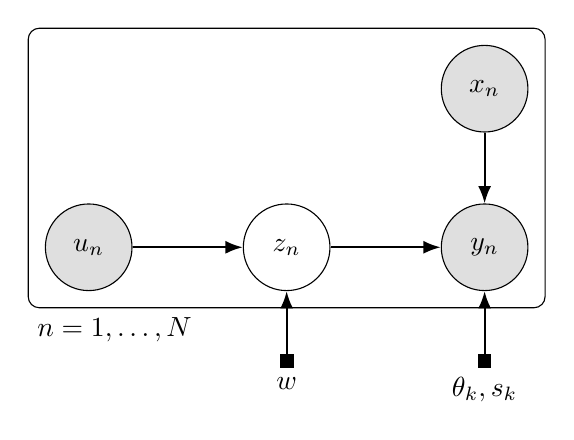
\begin{tikzpicture}[node distance=14mm]
\node[obs] (u) {$u_n$};
\node[lat,right=of u] (z) {$z_n$};
\node[obs,right=of z] (y) {$y_n$};
\node[obs,above=9mm of y] (x) {$x_n$};
\draw[edge] (u)--(z); \draw[edge] (z)--(y); \draw[edge] (x)--(y);
\node[par,below=8mm of z,label=below:{$w$}] (w) {}; \draw[edge] (w)--(z);
\node[par,below=8mm of y,label=below:{$\theta_k,s_k$}] (th) {}; \draw[edge] (th)--(y);
\begin{scope}[on background layer]
\node[plate,fit=(u)(z)(y)(x),label={[anchor=north west]south west:$n=1,\dots,N$}] {};
\end{scope}
\end{tikzpicture}
\end{center}

\paragraph{Complete-data likelihood.} With one-hot $z_n$,
\begin{equation}
p(Y,Z\mid X,U;\Psi)=\prod_{n=1}^N\prod_{k=1}^K\Big[\pi_k(u_n;w)\,\N\big(y_n;\mu_k(x_n;\theta_k),s_k^2\big)\Big]^{z_{nk}}.
\end{equation}
\paragraph{Observed-data log-likelihood.} Summing out each $z_n$ (Appendix A(c) shows the step) gives
\begin{equation}\label{eq:softmax-ll}
\ell(\Psi)=\log p(Y\mid X,U;\Psi)=\sum_{n=1}^N\log\sum_{k=1}^K\pi_k(u_n;w)\,\N\big(y_n;\mu_k(x_n;\theta_k),s_k^2\big).
\end{equation}
The sum inside the logarithm couples all the parameters, so there is no closed-form maximiser even when the experts are linear.

\subsection{Maximising it with EM}

\paragraph{E-step.} Using the current parameters $\Psi^{(q)}$, compute the responsibilities
\begin{equation}
\gamma_{nk}=p(z_{nk}=1\mid y_n,x_n,u_n;\Psi^{(q)})=\frac{\pi_k(u_n)\,\N\big(y_n;\mu_k(x_n),s_k^2\big)}{\sum_j\pi_j(u_n)\,\N\big(y_n;\mu_j(x_n),s_j^2\big)}.
\end{equation}
\paragraph{The $Q$-function} is the complete-data log-likelihood with each $z_{nk}$ replaced by $\gamma_{nk}$. It separates into a gate part and one part per expert:
\begin{equation}
Q(\Psi;\Psi^{(q)})=\underbrace{\sum_n\sum_k\gamma_{nk}\log\pi_k(u_n;w)}_{Q_{\text{gate}}(w)}+\sum_k\underbrace{\sum_n\gamma_{nk}\Big[-\tfrac12\log(2\pi s_k^2)-\frac{(y_n-\mu_k(x_n;\theta_k))^2}{2s_k^2}\Big]}_{Q_k(\theta_k,s_k)}.
\end{equation}
\paragraph{M-step.}
\begin{itemize}
  \item \emph{Gate.} $Q_{\text{gate}}$ is a cross-entropy with soft targets $\gamma_{nk}$, i.e.\ a weighted multinomial logistic regression. It is concave in $w$ and is solved by IRLS (Appendix A(g)).
  \item \emph{Experts.} For fixed $s_k$, maximising $Q_k$ over $\theta_k$ is \emph{weighted least squares}, $\min_{\theta_k}\sum_n\gamma_{nk}(y_n-\mu_k(x_n;\theta_k))^2$. For linear experts this has a closed form. For MLPs it does not, so one takes a few gradient steps. Doing so still increases $Q$, which is all EM needs: this is \emph{generalised EM}.
  \item \emph{Noise.} Setting $\partial Q_k/\partial s_k^2=0$ gives $s_k^2=\sum_n\gamma_{nk}(y_n-\mu_k(x_n))^2\big/\sum_n\gamma_{nk}$.
\end{itemize}

\subsection{Why EM never decreases the likelihood}

For \emph{any} distribution $q(Z)$ over the latent variables,
\begin{align}
\log p(Y\mid\Psi)&=\sum_Z q(Z)\log p(Y\mid\Psi)=\sum_Zq(Z)\log\frac{p(Y,Z\mid\Psi)}{p(Z\mid Y,\Psi)}\nonumber\\
&=\underbrace{\sum_Zq(Z)\log\frac{p(Y,Z\mid\Psi)}{q(Z)}}_{\mathcal L(q,\Psi)}\;+\;\underbrace{\sum_Zq(Z)\log\frac{q(Z)}{p(Z\mid Y,\Psi)}}_{\mathrm{KL}(q\,\|\,p(Z\mid Y,\Psi))\;\ge\;0}.
\end{align}
So $\mathcal L(q,\Psi)$ is a lower bound on the log-likelihood (Bishop \S9.4).
\begin{itemize}
  \item The \textbf{E-step} sets $q(Z)=p(Z\mid Y,\Psi^{(q)})$. The KL term becomes zero and the bound touches the log-likelihood at $\Psi^{(q)}$.
  \item With this $q$, $\mathcal L(q,\Psi)=Q(\Psi;\Psi^{(q)})-\sum_Zq\log q$. The second term does not depend on $\Psi$, so the \textbf{M-step}, which maximises $Q$, maximises the bound.
\end{itemize}
Therefore
\begin{equation}
\log p(Y\mid\Psi^{(q+1)})\;\ge\;\mathcal L(q,\Psi^{(q+1)})\;\ge\;\mathcal L(q,\Psi^{(q)})\;=\;\log p(Y\mid\Psi^{(q)}).
\end{equation}
Any $\Psi^{(q+1)}$ that merely \emph{increases} $Q$ keeps this chain of inequalities, which is why generalised EM still works.

\subsection{Why gradient training of the likelihood behaves like EM}

\paragraph{Fisher's identity.} The gradient of the observed-data log-likelihood equals the posterior expectation of the gradient of the complete-data log-likelihood:
\begin{equation}
\nabla_\Psi\log p(Y\mid\Psi)=\frac{\sum_Z\nabla_\Psi p(Y,Z\mid\Psi)}{p(Y\mid\Psi)}=\sum_Z\frac{p(Y,Z\mid\Psi)}{p(Y\mid\Psi)}\nabla_\Psi\log p(Y,Z\mid\Psi)=\E_{p(Z\mid Y,\Psi)}\big[\nabla_\Psi\log p(Y,Z\mid\Psi)\big].
\end{equation}
The right-hand side is exactly $\nabla_\Psi Q(\Psi;\Psi')$ evaluated at $\Psi'=\Psi$. \textbf{A gradient step on the log-likelihood is therefore an E-step (compute $\gamma$ with the current parameters) followed by one small step on the M-step objective.} EM and gradient ascent climb the same function and stop at the same kind of point, where the gradient is zero. EM jumps to the maximum of $Q$ when it can; gradient ascent takes small steps. With MLP experts we cannot jump anyway.

\paragraph{The gradients for one observation.} Write $\ell_n=\log\sum_k\pi_k\N_k$ with $\N_k=\N(y_n;\mu_k,s_k^2)$.
\begin{itemize}
  \item \emph{Expert mean.} Only the $k$-th term depends on $\mu_k$, and $\partial\log\N_k/\partial\mu_k=(y_n-\mu_k)/s_k^2$, so
  \begin{equation}\label{eq:grad-mu}
  \frac{\partial\ell_n}{\partial\mu_k}=\frac{\pi_k\N_k}{\sum_j\pi_j\N_j}\cdot\frac{y_n-\mu_k}{s_k^2}=\gamma_{nk}\,\frac{y_n-\mu_k}{s_k^2}.
  \end{equation}
  \item \emph{Expert noise.} Since $\partial\log\N_k/\partial\log s_k=-1+(y_n-\mu_k)^2/s_k^2$,
  \begin{equation}
  \frac{\partial\ell_n}{\partial\log s_k}=\gamma_{nk}\Big[\frac{(y_n-\mu_k)^2}{s_k^2}-1\Big].
  \end{equation}
  \item \emph{Gate logits} $a_k$, with $\pi=\softmax(a)$. Using \eqref{eq:softmax-deriv},
  \begin{equation}
  \frac{\partial\ell_n}{\partial a_k}=\sum_j\frac{\N_j}{\sum_l\pi_l\N_l}\,\pi_j(\delta_{jk}-\pi_k)=\gamma_{nk}-\pi_k\sum_j\gamma_{nj}=\gamma_{nk}-\pi_k.
  \end{equation}
\end{itemize}
Each gradient is the EM weighting in disguise. The expert that ``owns'' an observation (large $\gamma_{nk}$) receives its error signal, scaled by $1/s_k^2$. The gate is pulled towards the posterior $\gamma$, as in Weigend et al.\ (1995) eqs.~24--25. In our base case the gate is frozen, so only \eqref{eq:grad-mu} and the noise gradient are used.

\subsection{Backpropagation in depth}

Backpropagation is the chain rule applied efficiently to the expert MLP of Section 3, eqs.~\eqref{eq:pre}--\eqref{eq:out}. We minimise the loss $L_n=-\ell_n$ for one observation. Its derivative with respect to expert $k$'s output is, from \eqref{eq:grad-mu},
\begin{equation}
\delta^{\text{out}}_k:=\frac{\partial L_n}{\partial\mu_k}=-\gamma_{nk}\,\frac{y_n-\mu_k}{s_k^2}.
\end{equation}
Drop the index $k$ below: the same steps run inside every expert.

\paragraph{Step 1: forward pass.} Compute and \emph{store} $a^{(\ell)}$ and $h^{(\ell)}$ for $\ell=1,\dots,L$, then the output $\mu$, the responsibility $\gamma$ and $\delta^{\text{out}}$.

\paragraph{Step 2: output layer.} Since $\mu=w^{(L+1)\top}h^{(L)}+b^{(L+1)}$,
\begin{equation}
\frac{\partial L_n}{\partial w^{(L+1)}}=\delta^{\text{out}}\,h^{(L)},\qquad \frac{\partial L_n}{\partial b^{(L+1)}}=\delta^{\text{out}}.
\end{equation}

\paragraph{Step 3: define the error at every hidden layer,} $\delta^{(\ell)}:=\partial L_n/\partial a^{(\ell)}\in\R^{H_\ell}$. For the last hidden layer, $\mu$ depends on $a^{(L)}_m$ only through $h^{(L)}_m=g(a^{(L)}_m)$, so
\begin{equation}
\delta^{(L)}_m=\delta^{\text{out}}\,w^{(L+1)}_m\,g'\big(a^{(L)}_m\big),\qquad\text{i.e.}\qquad\delta^{(L)}=g'\big(a^{(L)}\big)\odot w^{(L+1)}\,\delta^{\text{out}}.
\end{equation}

\paragraph{Step 4: the backward recursion.} Layer $\ell$ affects the loss only through the pre-activations of layer $\ell+1$, $a^{(\ell+1)}_j=\sum_mW^{(\ell+1)}_{jm}\,g(a^{(\ell)}_m)+b^{(\ell+1)}_j$, so $\partial a^{(\ell+1)}_j/\partial a^{(\ell)}_m=W^{(\ell+1)}_{jm}\,g'(a^{(\ell)}_m)$. The chain rule sums over every path from $a^{(\ell)}_m$ to the loss:
\begin{equation}
\delta^{(\ell)}_m=\sum_{j=1}^{H_{\ell+1}}\delta^{(\ell+1)}_j\,W^{(\ell+1)}_{jm}\,g'\big(a^{(\ell)}_m\big)\qquad\Longleftrightarrow\qquad\delta^{(\ell)}=g'\big(a^{(\ell)}\big)\odot\Big(W^{(\ell+1)\top}\delta^{(\ell+1)}\Big).
\end{equation}

\paragraph{Step 5: weight gradients.} Since $a^{(\ell)}_j=\sum_mW^{(\ell)}_{jm}h^{(\ell-1)}_m+b^{(\ell)}_j$,
\begin{equation}
\frac{\partial L_n}{\partial W^{(\ell)}_{jm}}=\delta^{(\ell)}_j\,h^{(\ell-1)}_m\quad\Longleftrightarrow\quad\frac{\partial L_n}{\partial W^{(\ell)}}=\delta^{(\ell)}\,h^{(\ell-1)\top},\qquad\frac{\partial L_n}{\partial b^{(\ell)}}=\delta^{(\ell)}.
\end{equation}
Each gradient is ``error arriving at the unit'' times ``signal that entered the unit''.

\paragraph{A tiny example.} One hidden unit, squared-error loss: $f(x)=w_2\,g(w_1x+b_1)+b_2$, $a=w_1x+b_1$, $L=\frac12(y-f)^2$.
\begin{equation}
\frac{\partial L}{\partial w_2}=-(y-f)\,g(a),\quad\frac{\partial L}{\partial b_2}=-(y-f),\quad\frac{\partial L}{\partial w_1}=-(y-f)\,w_2\,g'(a)\,x,\quad\frac{\partial L}{\partial b_1}=-(y-f)\,w_2\,g'(a).
\end{equation}
The error $-(y-f)$ is computed once and reused, travelling backwards through $w_2$ and $g'$. That reuse is the whole trick.

\paragraph{Why this is efficient.} One backward pass costs about as much as one forward pass and returns the gradient with respect to \emph{all} parameters. Finite differences would need one extra forward pass per parameter. Reverse-mode automatic differentiation (PyTorch's autograd) carries out exactly Steps 1--5 for any graph we write down, including the mixture log-likelihood and the gate.

\paragraph{The update.} Average the gradients over a mini-batch $\mathcal B$ and step downhill:
\begin{equation}
\theta\leftarrow\theta-\eta\,\frac{1}{|\mathcal B|}\sum_{n\in\mathcal B}\nabla_\theta L_n.
\end{equation}
Adam, which the code uses, rescales each coordinate of this step by running estimates of the gradient's mean and root mean square. It is still a descent step on the same negative log-likelihood.

\paragraph{Three consequences for our base case.}
\begin{enumerate}
  \item \emph{Frozen base.} $f_0$ appears inside every $\mu_k$, but its parameters $\phi$ are excluded from the update, so the error stops at $f_0$.
  \item \emph{Zero-initialised final layer.} At step zero $w^{(L+1)}=0$, so $\delta^{(L)}=0$ and the hidden layers receive no gradient. They start learning one step later, once the final layer has moved.
  \item \emph{Mini-batches under the per-date likelihood.} The per-date likelihood (Section 7) couples all stocks of a date through the shared regime, so $\gamma$ must be computed over \emph{whole dates}. Mini-batches must therefore consist of complete dates. Under the per-row likelihood, which the study uses (Q24), any set of rows will do.
\end{enumerate}
\newpage

\section{From the softmax gate to the HMM gate}

\subsection{Three steps from Bishop's gate to ours}
\begin{enumerate}
  \item \textbf{The gate input becomes date-level.} Instead of the stock's own input, the gate sees the market history $\F_t$.
  \item \textbf{The latent becomes one per date and is shared.} A single $z_{t+1}$ governs every stock's return on day $t+1$ (Exercise A1(i), Chamroukhi \& Nguyen \S3).
  \item \textbf{The latent gets memory.} The prior of $z_{t+1}$ depends on $z_t$ through a transition matrix $A$, which makes the gate an HMM.
\end{enumerate}

\subsection{Why the Markov chain sits on the latent variables (Bishop \S13.1--13.2)}

\paragraph{Bishop \S13.1: a Markov chain on the observations.} The simplest way to give a series memory is
\begin{equation}
p(m_{t+1}\mid m_1,\dots,m_t)=p(m_{t+1}\mid m_t).
\end{equation}
This remembers a single step. A chain of order $M$ needs a number of parameters exponential in $M$, which is useless for regimes that last months.

\paragraph{Bishop \S13.2: put the chain on a hidden variable.} Let the hidden regime follow a first-order Markov chain, and let each observation depend only on the current regime:

\begin{center}
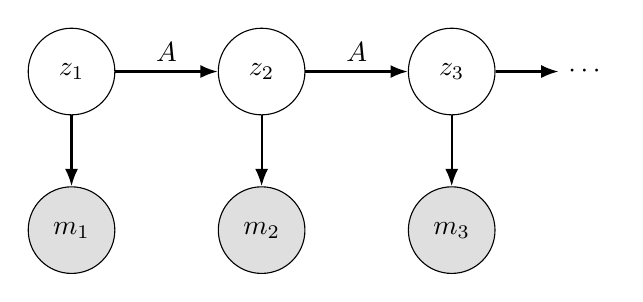
\begin{tikzpicture}[node distance=13mm]
\node[lat] (z1) {$z_1$}; \node[lat,right=of z1] (z2) {$z_2$}; \node[lat,right=of z2] (z3) {$z_3$}; \node[right=8mm of z3] (dots) {$\cdots$};
\node[obs,below=9mm of z1] (m1) {$m_1$}; \node[obs,below=9mm of z2] (m2) {$m_2$}; \node[obs,below=9mm of z3] (m3) {$m_3$};
\draw[edge] (z1)--node[above]{$A$}(z2); \draw[edge] (z2)--node[above]{$A$}(z3); \draw[edge] (z3)--(dots);
\draw[edge] (z1)--(m1); \draw[edge] (z2)--(m2); \draw[edge] (z3)--(m3);
\end{tikzpicture}
\end{center}

The observations are then \emph{not} Markov of any finite order. To predict $m_{t+1}$ one needs the belief about $z_t$, and that belief depends on the whole history $m_1,\dots,m_t$. The model has long memory with only $K(K-1)$ transition parameters.

\paragraph{The transition matrix.} In Bishop's notation (eq.~13.7), with one-hot regimes,
\begin{equation}
A_{jk}=p(z_{t+1}=k\mid z_t=j),\qquad 0\le A_{jk}\le1,\qquad\sum_{k=1}^KA_{jk}=1,\qquad p(z_{t+1}\mid z_t,A)=\prod_{j=1}^K\prod_{k=1}^KA_{jk}^{\,z_{tj}\,z_{t+1,k}}.
\end{equation}
Exactly one $z_{tj}$ and one $z_{t+1,k}$ equal $1$, so the double product picks out the single entry for the transition that happened. The first regime has its own distribution (Bishop eq.~13.8, where it is called $\pi$; we write $\rho$ because $\pi$ is our gate):
\begin{equation}
p(z_1\mid\rho)=\prod_k\rho_k^{\,z_{1k}}.
\end{equation}
The gate's parameters are $\theta_g=\{\rho,A,\nu_{1:K},\sigma_{1:K}\}$, the analogue of Bishop's $\theta=\{\pi,A,\phi\}$ in eq.~13.11. For $K=2$ that is $1+2+4=7$ numbers.

\paragraph{The HMM as a mixture model whose weights move (Bishop \S13.2).}
\begin{center}
\renewcommand{\arraystretch}{1.25}
\begin{tabularx}{\textwidth}{@{}llX@{}}
\toprule
Model & Mixing weight for observation $t+1$ & Depends on \\
\midrule
Gaussian mixture (Bishop ch.\ 9) & $\pi_k$, a constant & nothing \\
Mixture of experts (Bishop \S14.5) & $\pi_k(u)$, softmax gate & the input \\
HMM (Bishop \S13.2) & $A_{jk}$, row $j$ of $A$ & the previous regime \\
\textbf{Our HMM gate} & $\sum_jA_{jk}\,\xi_{t\mid t}(j)$ & the previous regime, averaged over our belief \\
\bottomrule
\end{tabularx}
\end{center}

\subsection{What $A$ does in the gate}

If we knew today's regime, tomorrow's mixing weights would be row $z_t$ of $A$. We do not know it, so we apply the sum rule over $z_t$ and then the Markov property:
\begin{equation}\label{eq:gate}
\boxed{\;\pi_k(t)=\mathbb P(z_{t+1}=k\mid\F_t)=\sum_{j=1}^Kp(z_{t+1}=k\mid z_t=j)\,\mathbb P(z_t=j\mid\F_t)=\sum_{j=1}^KA_{jk}\,\xi_{t\mid t}(j)\;}
\end{equation}
Inside the filter, $A$ is used every day in a \emph{predict} step, followed by a Bayes \emph{update} with the new market return. Write $\eta_{t}(k)=\N(m_{t};\nu_k,\sigma_k^2)$. Then
\begin{equation}
\xi_{t+1\mid t}(k)=\sum_jA_{jk}\,\xi_{t\mid t}(j)\quad\text{(predict)},\qquad\xi_{t+1\mid t+1}(k)=\frac{\xi_{t+1\mid t}(k)\,\eta_{t+1}(k)}{\sum_l\xi_{t+1\mid t}(l)\,\eta_{t+1}(l)}\quad\text{(update)}.
\end{equation}
So $A$ is the model's prior about how regimes move, and the market data correct it every day. The gate \eqref{eq:gate} is exactly the predict step.

\paragraph{What $A$ tells you.}
\begin{itemize}
  \item \emph{Persistence:} the diagonal $A_{kk}$ is the probability of staying in a regime.
  \item \emph{Expected duration:} each day the chain leaves regime $k$ with probability $1-A_{kk}$, so the time spent in $k$ is geometric. First-step analysis gives $\E[\text{duration}]=1/(1-A_{kk})$.
  \item \emph{Long-run share of time in each regime:} the stationary distribution, $\bar\rho A=\bar\rho$ with $\sum_k\bar\rho_k=1$.
  \item \emph{Forecasts $h$ days ahead:} $\mathbb P(z_{t+h}=k\mid\F_t)=[\xi_{t\mid t}\T A^h]_k$. These converge to $\bar\rho$; for $K=2$ the gap shrinks like $\lambda^h$, with $\lambda=A_{11}+A_{22}-1$ the second eigenvalue.
\end{itemize}

\paragraph{Worked example.}
\begin{equation}
A=\begin{pmatrix}0.98&0.02\\0.05&0.95\end{pmatrix}.
\end{equation}
\begin{itemize}
  \item Durations: calm lasts $1/0.02=50$ days on average, stressed lasts $1/0.05=20$ days.
  \item Stationary distribution: $0.02\,\bar\rho_1=0.05\,\bar\rho_2$ gives $\bar\rho=(5/7,\,2/7)\approx(0.71,\,0.29)$.
  \item Second eigenvalue: $\lambda=0.93$, so a regime forecast loses half of its distance to the long-run mix in $\ln0.5/\ln0.93\approx9.6$ days.
\end{itemize}

\subsection{How $A$ is estimated}

\paragraph{Step 1: if the regimes were observed.} The probability of a regime path depends on $A$ only through the transition counts $n_{jk}$:
\begin{equation}
p(z_{1:T}\mid A,\rho)=\rho_{z_1}\prod_{t=1}^{T-1}A_{z_tz_{t+1}}=\rho_{z_1}\prod_{j,k}A_{jk}^{\,n_{jk}}.
\end{equation}
Maximise the log subject to each row summing to one, with a Lagrange multiplier $\lambda_j$ per row:
\begin{equation}
\frac{\partial}{\partial A_{jk}}\Big[\sum_{j,k}n_{jk}\log A_{jk}+\sum_j\lambda_j\Big(1-\sum_kA_{jk}\Big)\Big]=\frac{n_{jk}}{A_{jk}}-\lambda_j=0\quad\Rightarrow\quad\hat A_{jk}=\frac{n_{jk}}{\sum_ln_{jl}}.
\end{equation}
So the estimate is a frequency: transitions from $j$ to $k$ divided by visits to $j$.

\paragraph{Step 2: the regimes are hidden, so use EM (Baum--Welch, Bishop \S13.2.1).} We replace the counts with their posterior expectations, which the forward--backward algorithm provides (next subsection):
\begin{equation}
\hat A_{jk}=\frac{\sum_{t=1}^{T-1}\xi_t(j,k)}{\sum_{t=1}^{T-1}\sum_l\xi_t(j,l)},\qquad\xi_t(j,k)=\mathbb P(z_t=j,z_{t+1}=k\mid\F_T).
\end{equation}

\subsection{The forward--backward recursion and how $\alpha$ and $\beta$ are used}

The recursion is needed in \textbf{Stage 1}, when the gate is fitted to the market series. Stage 2 does not need it, because there the gate prior is fixed for each date (Section 7).

\paragraph{The two quantities} (stated here without derivation; Bishop \S13.2.2):
\begin{align}
\alpha_t(k)&=p(m_1,\dots,m_t,\,z_t=k), & \alpha_1(k)&=\rho_k\eta_1(k), & \alpha_{t+1}(k)&=\eta_{t+1}(k)\textstyle\sum_j\alpha_t(j)A_{jk},\\
\beta_t(k)&=p(m_{t+1},\dots,m_T\mid z_t=k), & \beta_T(k)&=1, & \beta_t(j)&=\textstyle\sum_kA_{jk}\,\eta_{t+1}(k)\,\beta_{t+1}(k).
\end{align}
$\alpha$ looks at the past and today; $\beta$ looks at the future.

\paragraph{The five uses.}
\begin{enumerate}
  \item \emph{The likelihood:}
  \begin{equation}
  p(m_{1:T})=\sum_k\alpha_T(k)=\sum_k\alpha_t(k)\,\beta_t(k)\quad\text{for every }t.
  \end{equation}
  The second form gives a useful check that the code is correct.
  \item \emph{The filtered probability (the gate's ingredient):} $\xi_{t\mid t}(k)=\alpha_t(k)/\sum_j\alpha_t(j)$.
  \item \emph{The gate:} $\pi_k(t)=\sum_jA_{jk}\,\xi_{t\mid t}(j)$, eq.~\eqref{eq:gate}.
  \item \emph{The smoothed probability of a single regime:} $\gamma_t(k)=\mathbb P(z_t=k\mid\F_T)=\alpha_t(k)\,\beta_t(k)/p(m_{1:T})$.
  \item \emph{The smoothed probability of a transition:}
  \begin{equation}
  \xi_t(j,k)=\frac{\overbrace{\alpha_t(j)}^{\text{past, end in }j}\;\overbrace{A_{jk}}^{\text{jump}}\;\overbrace{\eta_{t+1}(k)}^{\text{tomorrow in }k}\;\overbrace{\beta_{t+1}(k)}^{\text{later data from }k}}{p(m_{1:T})}.
  \end{equation}
\end{enumerate}

\paragraph{The Baum--Welch loop.}
\begin{enumerate}
  \item \emph{Initialise} $\rho,A,\nu,\sigma$, e.g.\ $A$ with $0.9$ on the diagonal and the rest spread evenly.
  \item \emph{E-step:} forward and backward passes, then $\gamma_t(k)$ and $\xi_t(j,k)$.
  \item \emph{M-step}, all in closed form:
  \begin{equation}
  \rho_k=\gamma_1(k),\quad A_{jk}=\frac{\sum_{t=1}^{T-1}\xi_t(j,k)}{\sum_{t=1}^{T-1}\gamma_t(j)},\quad\nu_k=\frac{\sum_t\gamma_t(k)\,m_t}{\sum_t\gamma_t(k)},\quad\sigma_k^2=\frac{\sum_t\gamma_t(k)(m_t-\nu_k)^2}{\sum_t\gamma_t(k)}.
  \end{equation}
  \item \emph{Monitor} $\log p(m_{1:T})$, which EM never decreases (Section 4.4). Stop when it stops changing.
  \item \emph{Restart} from several initial values and keep the run with the highest likelihood.
\end{enumerate}

\paragraph{Scaling (Bishop \S13.2.4).} $\alpha_t$ is a product of $t$ densities and underflows. Work with normalised quantities instead:
\begin{equation}
\hat\alpha_t(k)=\xi_{t\mid t}(k),\qquad c_t=p(m_t\mid\F_{t-1}),\qquad\log p(m_{1:T})=\sum_{t=1}^T\log c_t,
\end{equation}
\begin{gather}
\hat\beta_T(k)=1,\qquad\hat\beta_t(j)=\frac{\sum_kA_{jk}\,\eta_{t+1}(k)\,\hat\beta_{t+1}(k)}{c_{t+1}},\\
\gamma_t(k)=\hat\alpha_t(k)\,\hat\beta_t(k),\qquad\xi_t(j,k)=\frac{\hat\alpha_t(j)\,A_{jk}\,\eta_{t+1}(k)\,\hat\beta_{t+1}(k)}{c_{t+1}}.
\end{gather}
The normalised forward pass is exactly the Hamilton filter. The Kim smoother used in \path{Model_Derivation_BaseCase.md} is another way of computing the same $\gamma_t$. Packages such as \texttt{statsmodels} maximise the same likelihood, with a few EM iterations followed by a numerical optimiser.

\begin{warnbox}{$\alpha$ is legal for forecasting, $\beta$ is not}
$\beta_t$ contains $m_{t+1},\dots,m_T$, so $\gamma_t$ and $\xi_t(j,k)$ are $\F_T$-measurable but not $\F_t$-measurable (Section 1.4). They may be used only inside the M-step on the \emph{training block}. The walk-forward procedure is therefore: fit Baum--Welch on the training block, freeze $\theta_g$, then run \emph{only the forward pass} through validation and test.
\end{warnbox}

\subsection{Initialising and labelling}
\begin{itemize}
  \item \emph{Simulating data.} Choose $A$ yourself (as in the example) and draw $z_{t+1}$ from the categorical distribution given by row $z_t$.
  \item \emph{Starting values for EM.} Use a heavy diagonal or random rows, with several restarts.
  \item \emph{Label switching.} Permuting the state labels permutes the rows and columns of $A$ and leaves the likelihood unchanged. To make ``state 1'' mean the same thing in every walk-forward fold, order the states after fitting, e.g.\ by $\sigma_k$ from low to high. The HMM is fitted first, so this ordering also fixes which expert is which.
\end{itemize}
\newpage

\section{The full generative model (base case)}

\subsection{The generative story}

Days run $t=1,\dots,T$. On each day the universe $\mathcal S_t$ is fixed at the close, characteristics $x_{i,t}$ are observed, and tomorrow's returns $r_{i,t+1}$ are the targets.

\begin{enumerate}
  \item \textbf{Regime.} $z_1\sim\text{Cat}(\rho)$. For $t\ge1$, tomorrow's regime is drawn from row $z_t$ of $A$:
  \begin{equation}
  z_{t+1}\mid z_t=j\ \sim\ \text{Cat}\big(A_{j1},\dots,A_{jK}\big).
  \end{equation}
  \item \textbf{Market.} The market return is drawn from the regime's Gaussian:
  \begin{equation}
  m_{t}\mid z_{t}=k\ \sim\ \N\big(\nu_k,\sigma_k^2\big).
  \end{equation}
  \item \textbf{Cross-section.} For every $i\in\mathcal S_t$, tomorrow's return is drawn from the expert of tomorrow's regime, with a mean set by the stock's characteristics today:
  \begin{equation}
  r_{i,t+1}\mid z_{t+1}=k,\ x_{i,t}\ \sim\ \N\big(\mu_k(x_{i,t}),\,s_k^2\big),\qquad\mu_k(x)=f_0(x)+c_k(x;\psi_k).
  \end{equation}
\end{enumerate}

\subsection{The graph}

\begin{center}
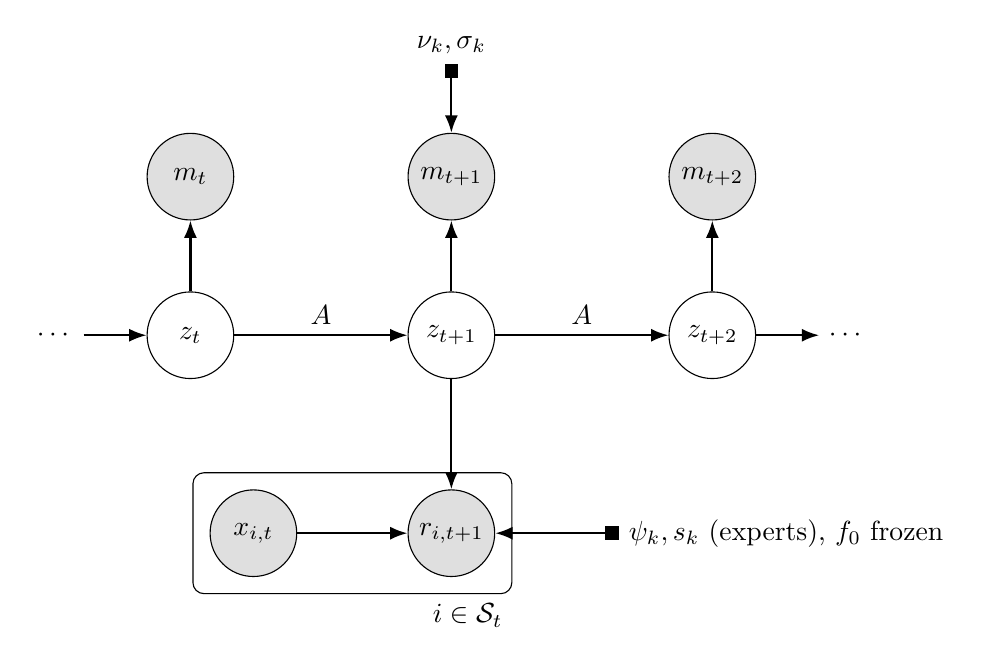
\begin{tikzpicture}[node distance=16mm]
\node[lat] (zt) {$z_t$};
\node[lat,right=22mm of zt] (zt1) {$z_{t+1}$};
\node[lat,right=22mm of zt1] (zt2) {$z_{t+2}$};
\node[left=8mm of zt] (dl) {$\cdots$}; \node[right=8mm of zt2] (dr) {$\cdots$};
\draw[edge] (dl)--(zt); \draw[edge] (zt)--node[above]{$A$}(zt1); \draw[edge] (zt1)--node[above]{$A$}(zt2); \draw[edge] (zt2)--(dr);
\node[obs,above=9mm of zt] (mt) {$m_t$};
\node[obs,above=9mm of zt1] (mt1) {$m_{t+1}$};
\node[obs,above=9mm of zt2] (mt2) {$m_{t+2}$};
\draw[edge] (zt)--(mt); \draw[edge] (zt1)--(mt1); \draw[edge] (zt2)--(mt2);
\node[obs,below=14mm of zt1] (r) {$r_{i,t+1}$};
\node[obs,left=14mm of r] (x) {$x_{i,t}$};
\draw[edge] (x)--(r); \draw[edge] (zt1)--(r);
\begin{scope}[on background layer]
\node[plate,fit=(x)(r),label={[anchor=north east]south east:{$i\in\mathcal S_t$}}] {};
\end{scope}
\node[par,right=14mm of r,label=right:{$\psi_k,s_k$ (experts), $f_0$ frozen}] (pe) {}; \draw[edge] (pe)--(r);
\node[par,above=7mm of mt1,label=above:{$\nu_k,\sigma_k$}] (pg) {}; \draw[edge] (pg)--(mt1);
\end{tikzpicture}
\end{center}

The model has two layers.
\begin{itemize}
  \item \textbf{The HMM layer:} a chain over days, in which each regime emits that day's market return.
  \item \textbf{The cross-section layer:} a plate over stocks. Each stock's return has two parents, the \emph{shared} regime of its day and its \emph{own} characteristics.
\end{itemize}
Equivalently, this is an HMM whose emission on day $t+1$ is the whole vector
\begin{equation*}
\big(m_{t+1},\,r_{1,t+1},\,\dots,\,r_{N_t,t+1}\big).
\end{equation*}
It is Chamroukhi \& Nguyen's HMM regression (\S4.2) with a vector-valued observation at each time point.

\subsection{Deriving the joint distribution}

Write $R$ for all returns $r_{i,t+1}$ ($t=1,\dots,T-1$, $i\in\mathcal S_t$) and $X$ for all characteristics.

\paragraph{Step 1: product rule} (always true):
\begin{equation}
p(z_{1:T},m_{1:T},R\mid X)=p(z_{1:T}\mid X)\;p(m_{1:T}\mid z_{1:T},X)\;p(R\mid m_{1:T},z_{1:T},X).
\end{equation}

\paragraph{Step 2: the regime path.} Two assumptions:
\begin{itemize}
  \item \textbf{A0 (exogenous characteristics):} $p(z_{1:T}\mid X)=p(z_{1:T})$.
  \item \textbf{A1 (Markov):} $p(z_{t+1}\mid z_{1:t})=p(z_{t+1}\mid z_t)$.
\end{itemize}
Using the chain rule and then A1,
\begin{equation}
p(z_{1:T})=p(z_1)\prod_{t=1}^{T-1}p(z_{t+1}\mid z_{1:t})\overset{\text{A1}}{=}p(z_1)\prod_{t=1}^{T-1}A_{z_tz_{t+1}}.
\end{equation}

\paragraph{Step 3: the market series.}
\begin{itemize}
  \item \textbf{A2 (market emission):} given its own day's regime, $m_t$ is independent of all other regimes, all other market returns and the characteristics.
\end{itemize}
\begin{equation}
p(m_{1:T}\mid z_{1:T},X)=\prod_{t=1}^Tp(m_t\mid m_{1:t-1},z_{1:T},X)\overset{\text{A2}}{=}\prod_{t=1}^T\N(m_t;\nu_{z_t},\sigma_{z_t}^2).
\end{equation}

\paragraph{Step 4: the cross-section.}
\begin{itemize}
  \item \textbf{A3 (cross-sectional emission):} given $z_{t+1}$ and its own $x_{i,t}$, $r_{i,t+1}$ is independent of (a) the other stocks' returns, (b) the market return $m_{t+1}$, (c) all other days' returns and (d) the regimes on other days.
\end{itemize}
\begin{equation}
p(R\mid m_{1:T},z_{1:T},X)\overset{\text{A3}}{=}\prod_{t=1}^{T-1}\prod_{i\in\mathcal S_t}\N\big(r_{i,t+1};\mu_{z_{t+1}}(x_{i,t}),s_{z_{t+1}}^2\big).
\end{equation}

\paragraph{Result.}
\begin{equation}\label{eq:joint}
\boxed{\begin{aligned}p(z_{1:T},m_{1:T},R\mid X)&=p(z_1)\prod_{t=1}^{T-1}A_{z_tz_{t+1}}\;\prod_{t=1}^{T}\N\big(m_t;\nu_{z_t},\sigma_{z_t}^2\big)\\&\quad\times\prod_{t=1}^{T-1}\prod_{i\in\mathcal S_t}\N\big(r_{i,t+1};\mu_{z_{t+1}}(x_{i,t}),s_{z_{t+1}}^2\big)\end{aligned}}
\end{equation}
This is Bishop's eq.~13.10 with one extra product over stocks inside each day. It can be read straight off the graph: one factor per node, each conditioned on its parents (Bishop eq.~8.5).

\subsection{What kind of quantity each symbol is}
\begin{center}
\renewcommand{\arraystretch}{1.25}
\begin{tabularx}{\textwidth}{@{}lX@{}}
\toprule
Role & Quantities \\
\midrule
Observed & market series $m_{1:T}$, stock returns $r_{i,t+1}$ \\
Conditioned on, not modelled & characteristics $x_{i,t}$, universe $\mathcal S_t$ \\
Latent & regimes $z_{1:T}$ \\
Gate parameters $\theta_g$ & $\rho$, $A$, $\nu_k$, $\sigma_k$ \\
Base parameters (frozen) & $\phi$ inside $f_0$ \\
Expert parameters & $\psi_k$ inside $c_k$, noise $s_k$ \\
\bottomrule
\end{tabularx}
\end{center}
The cross-section part of the model is \emph{discriminative}: it models returns given characteristics, never the characteristics themselves. The market part is \emph{generative}: it models the series itself.

\subsection{How realistic the assumptions are}
\begin{itemize}
  \item \textbf{A0} is mild. Characteristics such as momentum do vary with the regime, but we condition on them rather than use them to infer it. This is the design choice that keeps stock information out of the gate.
  \item \textbf{A1} carries the persistence. It implies geometric regime durations (Chamroukhi \& Nguyen \S4.3).
  \item \textbf{A2} holds for a plain Gaussian Hamilton model. The autoregressive version deliberately breaks it, which is the origin of the alignment bug G-2.
  \item \textbf{A3(b)} is the weak point for \emph{raw} returns. The market return is roughly the average of the stock returns, so on a $-4\%$ day almost every stock is down beyond what the regime explains. With the \emph{market-neutral} target the study uses (Q25) the common shock is removed and A3(b) becomes a reasonable approximation.
  \item \textbf{A3(a)} is only approximate, because industry peers stay correlated. This would make the per-date posterior of Section 7 overconfident, and is one reason the experts are trained on the per-row composite likelihood instead (Section 7.3, Q24).
  \item \textbf{A4 (homoskedastic experts):} $s_k$ is the same for every stock in regime $k$ (Section 3.3).
\end{itemize}

\paragraph{Base-case estimation} (Section 7). The gate parameters are fitted by maximum likelihood on the market series (Baum--Welch) and frozen. The expert parameters are then fitted by maximising the mixture likelihood of the returns. There are no penalties, no tempering and no joint fit.
\newpage

\section{The likelihood (base case)}

\subsection{What is maximised, and in what order}

The full model's likelihood is \eqref{eq:joint} with every regime summed out. The base case does not maximise this in one go. It maximises two pieces in sequence:
\begin{center}
\renewcommand{\arraystretch}{1.25}
\begin{tabularx}{\textwidth}{@{}lXllX@{}}
\toprule
Stage & Maximises & Parameters & Algorithm & Afterwards \\
\midrule
1 & $\log p(m_{1:T};\theta_g)$ & $\rho,A,\nu,\sigma$ & Baum--Welch (\S5.5) & frozen \\
2 & log-likelihood of the returns, gate fixed & $\psi_k,s_k$ & gradient ascent (\S7.3) & --- \\
\bottomrule
\end{tabularx}
\end{center}
The Stage 1 objective is computed by the scaled forward pass:
\begin{equation}
\ell_{\text{gate}}(\theta_g)=\log p(m_{1:T};\theta_g)=\sum_{t=1}^T\log c_t.
\end{equation}

\subsection{The Stage 2 likelihood: summing out the regime date by date}

Fix a date $t$. Tomorrow's cross-section depends on the unknown $z_{t+1}$. Apply the sum rule over $z_{t+1}$ and then A3, which makes the stocks independent given the regime:
\begin{align}
p\big(r_{\cdot,t+1}\mid x_{\cdot,t},\F_t\big)&=\sum_{k=1}^K\mathbb P(z_{t+1}=k\mid\F_t)\;p\big(r_{\cdot,t+1}\mid x_{\cdot,t},z_{t+1}=k\big)\nonumber\\
&=\sum_{k=1}^K\pi_k(t)\prod_{i\in\mathcal S_t}\N\big(r_{i,t+1};\mu_k(x_{i,t}),s_k^2\big).
\end{align}
Taking logs and adding over dates gives the \textbf{per-date likelihood}:
\begin{equation}\label{eq:ldate}
\boxed{\;\ell_{\text{date}}(\psi,s)=\sum_{t=1}^{T-1}\log\sum_{k=1}^K\pi_k(t)\prod_{i\in\mathcal S_t}\N\big(r_{i,t+1};\mu_k(x_{i,t}),s_k^2\big)\;}
\end{equation}

\paragraph{Why adding over dates is allowed.} The gate is frozen and $\F_t$-measurable, i.e.\ built from the market alone. So the returns on one date never change the regime belief used on another date, and each date's term stands alone. Formally, \eqref{eq:ldate} is a \emph{cut} (composite) likelihood: the flow of information from returns back into the regime belief is deliberately removed. This is also why Stage 2 needs no forward--backward recursion.

\paragraph{What the full joint fit would do instead (not used).} Treat
\begin{equation*}
e_{t+1}(k)=\eta_{t+1}(k)\prod_{i\in\mathcal S_t}\N(r_{i,t+1};\mu_k,s_k^2)
\end{equation*}
as the emission and run forward--backward over everything. In log terms, the product over roughly 500 stocks outweighs the single market term by a factor of hundreds. The cross-section would then decide what the regimes are, and their meaning as \emph{market} regimes would be lost. The base case avoids this by design.

\paragraph{Numerics.} Compute
\[
\log\sum_k\exp\Big(\log\pi_k(t)+\sum_{i\in\mathcal S_t}\log\N_{ik}\Big)
\]
with a single \texttt{logsumexp}. Never multiply densities directly.

\subsection{The objective used: the per-row composite likelihood (Q24, decided)}

The study does \emph{not} maximise $\ell_{\text{date}}$. It maximises
\begin{equation}\label{eq:lrow}
\boxed{\;\ell_{\text{row}}(\psi,s)=\sum_{t=1}^{T-1}\sum_{i\in\mathcal S_t}\log\sum_{k=1}^K\pi_k(t)\,\N\big(r_{i,t+1};\mu_k(x_{i,t}),s_k^2\big)\;}
\end{equation}
(decided 2026-10-05, Q24). This section gives the short version; Appendix~\ref{app:perrow} gives the full theory, step by step. There are two ways to read this objective.

\paragraph{Reading 1: the likelihood of a different model.} If every stock-day drew its own regime from the day's prior, \eqref{eq:lrow} would be that model's exact likelihood. In the graph of Section 6 the latent node would move inside the stock plate.

\paragraph{Reading 2: a composite likelihood of \emph{our} model.} Keep the model of Section 6, with one regime per day, and ask for the distribution of a single stock's return on its own. Integrating out all other stocks (each integrates to one given $z_{t+1}$) and then $z_{t+1}$ gives
\begin{equation}
p\big(r_{i,t+1}\mid x_{i,t},\F_t\big)=\sum_{k=1}^K\pi_k(t)\,\N\big(r_{i,t+1};\mu_k(x_{i,t}),s_k^2\big).
\end{equation}
This is exactly the term inside \eqref{eq:lrow}. So $\ell_{\text{row}}$ is the sum of the \emph{correct} marginal log-likelihoods of the per-date model: it keeps every stock's own distribution and discards only the dependence between stocks on the same date. Such an objective is a \emph{composite likelihood}, in this case the \emph{independence likelihood} (Lindsay 1988; Varin, Reid \& Firth 2011).

\paragraph{Why it is a valid estimator.} Each term is a true log-density, so its score has expectation zero at the true parameters. A sum of unbiased score terms is an unbiased estimating equation, and under the usual regularity conditions its maximiser is consistent. The cost is efficiency, because the joint information carried by the co-movement of stocks on a date is not used, and its curvature does not give valid standard errors. Neither matters here: inference in the study comes from walk-forward rank ICs, not from the likelihood. Composite likelihood is used in finance for exactly this kind of large cross-section, where the full likelihood is unreliable (Pakel, Shephard, Sheppard \& Engle 2021).

\paragraph{Why it is preferred to $\ell_{\text{date}}$.}
\begin{enumerate}
  \item \textbf{Robustness to A3.} $\ell_{\text{date}}$ uses its extra information only through A3(a): given the regime, the stocks are independent. That assumption is false, because industry peers share shocks after the market is removed, and the market-neutral target leaves residual beta exposure (Q25). $\ell_{\text{date}}$ then counts correlated stocks as independent evidence about the regime. With $m$ stocks per cluster correlated at $\rho$, the cross-section carries the information of only
  \begin{equation*}
  N_{\text{eff}}\approx\frac{N}{1+(m-1)\rho}
  \end{equation*}
  independent stocks (Kish's design effect). For example, $N=500$, $m=45$ and $\rho=0.1$ give $N_{\text{eff}}\approx93$, so the per-date posterior would be overconfident by a factor of about five. $\ell_{\text{row}}$ needs only the marginals to be right, so this violation does not bias it (Liang \& Zeger 1986).
  \item \textbf{The gate stays in charge.} Under $\ell_{\text{date}}$ the responsibility $\gamma_t(k)$ is almost always $0$ or $1$ and is set by the day's returns (see the sharpness calculation below), so the cross-section re-decides the regime every day. Under $\ell_{\text{row}}$ one stock carries little evidence, so $\gamma_{i,t}(k)$ stays close to $\pi_k(t)$, and each expert learns mainly from the days that the \emph{gate} assigns to its regime. That is the point of freezing the gate (Q19): the regimes remain \emph{market} regimes.
  \item \textbf{Practicalities.} It is what the code already implements (\texttt{losses.mixture\_nll}, a log-sum-exp per row); mini-batches may be any rows; training is smoother.
\end{enumerate}

\paragraph{Its weakness, and the diagnostic.} The experts specialise less sharply, and the expert with the larger $s_k$ can drift into absorbing outlying stock-days instead of representing a regime. After training, check whether each expert's share of the training weight follows the gate's $\pi_k(t)$ or the size of the residuals.

\subsection{How Stage 2 is maximised}

\paragraph{The EM view.} The E-step gives each stock-day's posterior over the regime after seeing its own return:
\begin{equation}
\gamma_{i,t}(k)=\frac{\pi_k(t)\,\N\big(r_{i,t+1};\mu_k(x_{i,t}),s_k^2\big)}{\sum_j\pi_j(t)\,\N\big(r_{i,t+1};\mu_j(x_{i,t}),s_j^2\big)}.
\end{equation}
In the M-step each expert solves a weighted least-squares problem, with weight $\gamma_{i,t}(k)$ on row $(i,t)$, and the noise has a closed form:
\begin{equation}
\min_{\psi_k}\sum_t\sum_{i\in\mathcal S_t}\gamma_{i,t}(k)\big(r_{i,t+1}-\mu_k(x_{i,t};\psi_k)\big)^2,\qquad s_k^2=\frac{\sum_t\sum_i\gamma_{i,t}(k)\big(r_{i,t+1}-\mu_k(x_{i,t})\big)^2}{\sum_t\sum_i\gamma_{i,t}(k)}.
\end{equation}
With linear experts the first problem has a closed form (Appendix A(i)); with MLPs it does not.

\paragraph{What is actually done: gradient ascent on $\ell_{\text{row}}$.} By Fisher's identity (Section 4.5) the gradients carry the same weights:
\begin{equation}
\frac{\partial\ell_{\text{row}}}{\partial\mu_k(x_{i,t})}=\gamma_{i,t}(k)\,\frac{r_{i,t+1}-\mu_k(x_{i,t})}{s_k^2},\qquad\frac{\partial\ell_{\text{row}}}{\partial\log s_k}=\sum_t\sum_i\gamma_{i,t}(k)\Big[\frac{(r_{i,t+1}-\mu_k)^2}{s_k^2}-1\Big].
\end{equation}
Each step recomputes $\gamma$ with the current parameters and moves a little on the weighted problem. Backpropagation (Section 4.6) carries the first gradient into every expert's weights. Mini-batches may contain any rows.

\paragraph{Numerics.} For each row compute $\log\sum_k\exp\big(\log\pi_k(t)+\log\N_{ik}\big)$ with a single \texttt{logsumexp}.

\subsection{For comparison: how sharp the per-date posterior is}
Under $\ell_{\text{date}}$ the E-step pools the whole cross-section:
\begin{equation}
\log\frac{\gamma_t(k)}{\gamma_t(j)}=\log\frac{\pi_k(t)}{\pi_j(t)}+\sum_{i\in\mathcal S_t}\log\frac{\N(r_{i,t+1};\mu_k,s_k^2)}{\N(r_{i,t+1};\mu_j,s_j^2)}.
\end{equation}
If regime $k$ is true, each term of the sum has expectation equal to a Kullback--Leibler divergence, which is positive, so the sum grows roughly in proportion to $N_t$. For example, two experts that differ only in noise level ($1.5\%$ against $1\%$) give
\begin{equation}
\mathrm{KL}\big(\N(0,1.5^2)\,\|\,\N(0,1^2)\big)=\log\tfrac{1}{1.5}+\tfrac{1.5^2}{2}-\tfrac12\approx0.22\text{ nats per stock},
\end{equation}
so about 110 nats on a day with 500 stocks. The per-date $\gamma$ is therefore nearly always $0$ or $1$, whereas the per-row $\gamma$ stays close to the prior.

\begin{center}
\renewcommand{\arraystretch}{1.25}
\begin{tabularx}{\textwidth}{@{}lXX@{}}
\toprule
 & Per date $\ell_{\text{date}}$ & Per row $\ell_{\text{row}}$ (\textbf{used}) \\
\midrule
Relation to Section 6 & exact likelihood & composite (independence) likelihood \\
Needs A3(a) & yes & no, only correct marginals \\
Responsibilities & near $0/1$, set by the day's returns & soft, close to the gate's $\pi$ \\
Experts specialise by & days whose cross-section fits & the gate's regimes (risk: tail rows) \\
Mini-batches & whole dates & any rows \\
Forecast formula & $\sum_k\pi_k\mu_k$ & identical \\
\bottomrule
\end{tabularx}
\end{center}
The forecast formula is the same under both, because forecasts use $\pi$ and never $\gamma$; only the training of the experts differs.

\subsection{What freezing the gate changes}
\begin{itemize}
  \item No gradient reaches the gate. The $\pi_k(t)$ are fixed numbers, and the experts adapt to them.
  \item The HMM fixes the labels: expert $k$ is the expert for HMM state $k$, in the order chosen in Section 5.6.
  \item On a given day the experts can still ``disagree'' with the gate, because $\gamma$ uses the returns and $\pi$ does not. A scatter of $\pi$ against $\gamma$ (Weigend et al.\ 1995) shows how informative the gate is.
  \item Freezing causes no look-ahead: Baum--Welch runs on the training block only, and only the forward pass runs after it.
\end{itemize}
\newpage

\section{Prediction and posteriors (base case)}

\subsection{The information at forecast time}
At the close of day $t$ the forecast may use $\mathcal G_t$: the market history (through the forward pass only), today's characteristics $x_{i,t}$, and the frozen parameters. The gate is the $\F_t$-measurable probability
\begin{equation}
\pi_k(t)=\mathbb P(z_{t+1}=k\mid\F_t)=\sum_jA_{jk}\,\xi_{t\mid t}(j).
\end{equation}

\subsection{The predictive distribution of one stock}
Apply the sum rule over $z_{t+1}$:
\begin{equation}\label{eq:pred}
p\big(r_{i,t+1}\mid x_{i,t},\F_t\big)=\sum_{k=1}^K\pi_k(t)\,\N\big(r_{i,t+1};\mu_k(x_{i,t}),s_k^2\big).
\end{equation}
This is a Gaussian mixture, so it can be skewed and fat-tailed even though every expert is Gaussian. It is the full forecast; everything below summarises it.

\subsection{The point forecast}
By the law of total expectation,
\begin{equation}
\hat r_{i,t+1}=\E\big[r_{i,t+1}\mid x_{i,t},\F_t\big]=\sum_k\pi_k(t)\,\mu_k(x_{i,t})=f_0(x_{i,t})+\sum_k\pi_k(t)\,c_k(x_{i,t}).
\end{equation}
The last step uses $\sum_k\pi_k(t)=1$: the base comes out of the sum, so the forecast is the base plus the gate-weighted corrections. The rank IC is computed from $\hat r_{i,t+1}$.

\subsection{The predictive variance}
The second moment is $\E[r^2\mid\cdot]=\sum_k\pi_k(s_k^2+\mu_k^2)$. Subtracting $\hat r^{\,2}$ and rearranging gives the law of total variance:
\begin{equation}
\Var\big(r_{i,t+1}\mid x_{i,t},\F_t\big)=\underbrace{\sum_k\pi_k(t)\,s_k^2}_{\text{noise within a regime}}+\underbrace{\sum_k\pi_k(t)\big(\mu_k(x_{i,t})-\hat r_{i,t+1}\big)^2}_{\text{experts disagree, regime uncertain}}.
\end{equation}
The first term remains even if tomorrow's regime were known. The second exists only because the regime is unknown and the experts predict different things; it vanishes if the gate is certain or if the experts agree for this stock.

\subsection{Covariance between stocks (per-date model)}
Two stocks share $z_{t+1}$ and are independent given it, so uncertainty about the regime makes them co-move:
\begin{equation}
\Cov\big(r_{i,t+1},r_{j,t+1}\mid\cdot\big)=\sum_k\pi_k\,\mu_k(x_{i,t})\,\mu_k(x_{j,t})-\hat r_{i,t+1}\hat r_{j,t+1}=\sum_k\pi_k(t)\big(\mu_k(x_{i,t})-\hat r_{i,t+1}\big)\big(\mu_k(x_{j,t})-\hat r_{j,t+1}\big).
\end{equation}
This covariance is a property of the model; it is not affected by training with the per-row objective (Q24), which only discards it from the estimation. Under the alternative per-row \emph{model} it would be zero. It matters only for portfolios built from the predictive distribution; ranking uses $\hat r$ alone.

\subsection{The study's horizon: $h=5$}
The study uses a daily gate, a daily cross-section and a 5-day target (Q21, decided 2026-10-05). The derivations in these notes are written for one step, with $r_{i,t+1}$; in the study that step is the 5-day window $(t,t+5]$, and $r_{i,t+1}$ stands for the market-neutral return over it. The regime can change inside the window, and the regime forecast $j$ days ahead is $\mathbb P(z_{t+j}=k\mid\F_t)=[\xi_{t\mid t}\T A^j]_k$. The likelihood keeps a single regime for the whole window, which is a reasonable approximation because 5 days is short against typical regime durations of 20--50 days (Section 5.3); the window-average weight below makes the point forecast exact even when the regime changes inside the window. The gate weight for the window is the average of the $j=1,\dots,5$ forecasts (decided 2026-10-05, Q27; Section~\ref{sec:predfilt}). Consecutive daily targets overlap by four days: statistics are overlap-corrected (Hansen--Hodrick), and the training likelihood is used for estimation, not inference.

\subsection{Every regime probability, and where it may be used}
\begin{center}
\small\renewcommand{\arraystretch}{1.3}
\begin{tabularx}{\textwidth}{@{}p{2.6cm}p{1.6cm}p{2.6cm}Xp{1.4cm}@{}}
\toprule
Quantity & Measurable w.r.t. & Computed from & Used for & At forecast time \\
\midrule
filtered $\xi_{t\mid t}$ & $\F_t$ & forward pass ($\hat\alpha_t$) & building the gate & yes \\
gate $\bar w_k(t)$ ($=\pi_k(t)$ if $h=1$) & $\F_t$ & $\xi_{t\mid t}$ and $A$ & weighting the experts & yes \\
smoothed $\gamma_t$ (gate) & $\F_T$ & $\hat\alpha_t\hat\beta_t$ & Baum--Welch M-step, training block & \textbf{no} \\
pairwise $\xi_t(j,k)$ & $\F_T$ & $\hat\alpha,A,\eta,\hat\beta$ & updating $A$, training block & \textbf{no} \\
responsibility $\gamma_{i,t}(k)$ & $\mathcal G_{t+1}$ & Bayes per stock-day, uses $r_{i,t+1}$ & weighting expert gradients in training & \textbf{no} \\
\bottomrule
\end{tabularx}
\end{center}

\subsection{Why smoothed probabilities leak the future}
\begin{equation}
\gamma_t(k)\propto\alpha_t(k)\,\beta_t(k),\qquad\beta_t(k)=p(m_{t+1},\dots,m_T\mid z_t=k).
\end{equation}
Suppose the market crashes on day $t+3$. That crash is far more likely under the stressed regime, so $\beta_t$ shifts weight to the stressed regime on day $t$, three days before the crash, when no past data pointed to it. A gate built on smoothed probabilities therefore enters crashes in advance: the backtest looks excellent and means nothing. In the language of Section 1.4, the smoothed probability is not $\F_t$-measurable, so a forecast built on it is not adapted.

\paragraph{Leaks that are easy to miss.}
\begin{itemize}
  \item Refitting Baum--Welch on data that include validation or test dates. The M-step uses smoothed posteriors, so future data enter $\theta_g$.
  \item Training on smoothed weights and testing on filtered ones. This is not look-ahead at test time, but the experts face a different kind of input than they were trained on. That is why the filtered series is used on training dates too.
  \item Using the responsibilities $\gamma$ as features at forecast time. They contain the target itself.
  \item The purge gap (Q22, open). The forward pass must be carried continuously through the dates removed between training and test.
\end{itemize}

\subsection{The gate weight for an $h$-day target (Q27, decided)}\label{sec:predfilt}
Three $\F_t$-measurable candidates are available at the close of day $t$, all built from the filtered probability:
\begin{itemize}
  \item the \emph{filtered} probability $\xi_{t\mid t}(k)$, today's regime (used by \path{Model_Derivation_BaseCase.md} before this decision, and by the code's Hamilton gate);
  \item the \emph{one-step predicted} probability $\pi_k(t)=[\xi_{t\mid t}\T A]_k$, tomorrow's regime (Section 6 with $h=1$);
  \item the \emph{window average}, the expected share of the window $(t,t+h]$ spent in regime $k$:
\end{itemize}
\begin{equation}\label{eq:wbar}
\bar w_k(t)=\frac1h\sum_{j=1}^{h}\big[\xi_{t\mid t}\T A^{\,j}\big]_k.
\end{equation}

\paragraph{Why the window average is exact for the point forecast.} The target is the sum of $h$ daily returns. Suppose each day's expected return is set by that day's regime, with regime $k$ contributing $\mu_k(x_{i,t})/h$ per day. By the law of total expectation, day by day,
\begin{equation}
\E\big[y_{i,t}\mid\F_t\big]=\sum_{j=1}^h\sum_k\mathbb P\big(z_{t+j}=k\mid\F_t\big)\frac{\mu_k(x_{i,t})}{h}=\sum_k\bar w_k(t)\,\mu_k(x_{i,t}).
\end{equation}
So the gate-weighted forecast with \eqref{eq:wbar} is exactly the expected $h$-day return. The expected within-regime noise also adds up over days and is matched in the same way. The filtered weight assumes the regime never changes during the window, and the one-step weight assumes it changes at most once. For $h=1$, \eqref{eq:wbar} reduces to the one-step predicted probability, so every one-step formula in these notes is the $h=1$ case of this rule.

\paragraph{How large the differences are.} With the example $A$ of Section 5.3 and a filtered belief of certain stress, the weight on stress is $1.00$ (filtered), $0.95$ (one-step) and $0.86$ (window average with $h=5$). A descriptive fit of a two-state Hamilton model to the CRSP S\&P~500 index, 2015--2024, gives an average gap of $0.055$ between the filtered and window-average weights on the stressed regime, with a maximum of $0.10$. The gap is largest when the filter is sure of stress, because stress tends to end.

\paragraph{Decision.} The window average is used on training and test dates alike (Q27, decided 2026-10-05). Costs accepted: slightly softer weights, and dependence on a well-estimated $A$, whose errors compound over $h$ steps. The likelihood with these weights remains the one-regime-per-window approximation: the exact distribution of an $h$-day return is a mixture over regime \emph{paths}.
\newpage

\section{Assumptions and design checklist (base case)}

\subsection{Modelling assumptions}
\begin{center}
\renewcommand{\arraystretch}{1.3}
\begin{tabularx}{\textwidth}{@{}lXX@{}}
\toprule
 & Assumption & Comment \\
\midrule
A0 & Characteristics carry no information about the regime path & keeps stock information out of the gate \\
A1 & First-order Markov regimes with one $A$ per training block & geometric durations; $A$ re-estimated in every walk-forward fold \\
A2 & The market return depends only on its own day's regime (Gaussian, switching mean and variance) & the AR variant breaks it on purpose (G-2) \\
A3 & Given $z_{t+1}$ and $x_{i,t}$, the stock returns are independent of each other, of $m_{t+1}$ and of other days & weak for raw returns (common market shock); reasonable for the market-neutral target used here; industry peers remain correlated, which the per-row objective tolerates (Q24) \\
A4 & One noise level $s_k$ per regime, the same for all stocks & no stock-specific volatility in the experts \\
A5 & All parameters constant within a training block & re-estimated per fold \\
\bottomrule
\end{tabularx}
\end{center}

\subsection{Design choices and their status}
``Decided'' means decided for the base case or recorded as resolved in \path{Advisor_Questions.md}. ``Open'' gives the question number.
\begin{center}
\small\renewcommand{\arraystretch}{1.3}
\begin{tabularx}{\textwidth}{@{}p{4.2cm}Xp{3.3cm}@{}}
\toprule
Item & Base-case choice or options & Status \\
\midrule
Gate fitted separately and frozen & Baum--Welch on the training block, forward pass afterwards & decided (Q19) \\
Base pre-trained and frozen & $f_0$ fitted first, never updated & decided (Q7) \\
Filtered, never smoothed, as the basis of the gate & on training and test dates alike & decided (base-case derivation) \\
Gate weight for the $h$-day target & window average $\bar w_k(t)$ of the $1$- to $h$-step-ahead probabilities (Section 8.9) & decided (Q27) \\
Number of regimes $K$ & e.g.\ 2 or 3 & \textbf{open} (Q18) \\
Gate series $m_t$ & CRSP value-weighted S\&P 500 index, daily log return; filter runs through the purge gap & \textbf{decided} (Q23, Q22) \\
Frequency and horizon $h$ & daily gate, daily cross-section, $h=5$ (overlapping targets) & decided (Q21) \\
Filter through the purge gap & run forward continuously or restart & \textbf{open} (Q22) \\
Likelihood for the experts & $\ell_{\text{row}}$, the composite likelihood of the per-date model (Section 7.3) & decided (Q24) \\
Objective & base case: mixture log-likelihood only & decided here; Q20 open for the thesis \\
State labelling across folds & order states, e.g.\ by $\sigma_k$ & to check in code \\
Residual form & $\mu_k=f_0+c_k$, final layer of $c_k$ zero-initialised & implemented; Q6 and Q14 open \\
Expert noise $s_k$ & learned scalar per expert, frozen for the first 100 steps & implemented; no floor or prior in the base case \\
Regime information & enters only through the gate; experts see $x_{i,t}$ only & decided \\
Target & market-neutral return: forward return minus the date's equal-weighted cross-sectional mean & decided (Q25); not yet implemented \\
Expert and base architecture & MLP widths and depth & \textbf{open} (Q8; depth grid per Q11) \\
Training window and weighting & full block vs decay; crash preservation & \textbf{open} (Q16, B-2) \\
Hidden-layer initialisation & switch X-1 & \textbf{open} \\
Mini-batching & any rows (under $\ell_{\text{row}}$) & decided (Q24) \\
\bottomrule
\end{tabularx}
\end{center}

\subsection{The base case in one paragraph}
A $K$-state Gaussian HMM is fitted by Baum--Welch to the daily market series on the training block and frozen. Its forward pass gives, at the close of each day $t$, the filtered probability $\xi_{t\mid t}$; the gate weight for the 5-day target is its window average $\bar w_k(t)$ \eqref{eq:wbar}, which equals $\pi_k(t)=\mathbb P(z_{t+1}=k\mid\F_t)$ when $h=1$ (Q27). A frozen base MLP $f_0$ and $K$ zero-initialised MLP corrections $c_k$ define expert means $\mu_k=f_0+c_k$ with noise levels $s_k$. The corrections and noise levels are fitted by gradient ascent on the per-row (composite) mixture log-likelihood of tomorrow's returns with the gate held fixed (Q24). The forecast is $\hat r_{i,t+1}=f_0(x_{i,t})+\sum_k\pi_k(t)\,c_k(x_{i,t})$, and its full predictive distribution is the mixture \eqref{eq:pred}.
\newpage

\appendix
\section{Solution to Exercise A1}

Throughout, $\N_{nk}:=\N(y_n;\beta_k\T x_n,s_k^2)$ and $\pi_{nk}:=\pi_k(x_n;w)$.

\paragraph{(a) Generative story and graph.} For each $n$: given $x_n$, draw the expert label, then the target,
\begin{equation*}
z_n\sim\text{Cat}(\pi_{n1},\dots,\pi_{nK}),\qquad y_n\sim\N\big(\beta_{z_n}\T x_n,\,s_{z_n}^2\big).
\end{equation*} The graph is the one in Section 4.2 with $u_n=x_n$. Observed: $x_n,y_n$. Latent: $z_n$. Parameters: $w$ (entering at $z_n$) and $\beta_k,s_k$ (entering at $y_n$). The plate is over $n$, so the $z_n$ are independent across observations.

\paragraph{(b) Complete-data likelihood.} Exactly one $z_{nk}=1$ for each $n$, so
\begin{equation}
p(Y,Z\mid X;\Psi)=\prod_{n=1}^N\prod_{k=1}^K\big[\pi_{nk}\,\N_{nk}\big]^{z_{nk}},\qquad\log L_c(\Psi)=\sum_{n=1}^N\sum_{k=1}^Kz_{nk}\big[\log\pi_{nk}+\log\N_{nk}\big].
\end{equation}

\paragraph{(c) Observed-data log-likelihood.} Summing over $Z$ means summing over every $z_n$. The factor for observation $n$ depends only on $z_n$, so the sum moves inside the product. This is what fails in an HMM, where transitions link neighbouring latents:
\begin{equation}
p(Y\mid X;\Psi)=\sum_{z_1}\cdots\sum_{z_N}\prod_n\prod_k\big[\pi_{nk}\N_{nk}\big]^{z_{nk}}=\prod_n\sum_{z_n}\prod_k\big[\pi_{nk}\N_{nk}\big]^{z_{nk}}=\prod_n\sum_k\pi_{nk}\N_{nk}.
\end{equation}
The last step holds because, when $z_n$ has its $1$ in position $j$, every factor with $k\ne j$ equals $1$. Hence
\begin{equation}
\log L(\Psi)=\sum_{n=1}^N\log\sum_{k=1}^K\pi_k(x_n;w)\,\N(y_n;\beta_k\T x_n,s_k^2).
\end{equation}
The sum inside the logarithm couples $w$, every $\beta_k$ and every $s_k$, and the function is not concave. Setting the gradient to zero gives equations in which the responsibilities themselves depend on all the parameters, so there is no closed-form solution.

\paragraph{(d) E-step.} By Bayes' rule,
\begin{equation}
\tau_{nk}^{(q)}=p(z_{nk}=1\mid y_n,x_n;\Psi^{(q)})=\frac{p(z_{nk}=1\mid x_n)\,p(y_n\mid x_n,z_{nk}=1)}{p(y_n\mid x_n)}=\frac{\pi_{nk}^{(q)}\N_{nk}^{(q)}}{\sum_j\pi_{nj}^{(q)}\N_{nj}^{(q)}}.
\end{equation}

\paragraph{(e) The $Q$-function.} $\log L_c$ is linear in $z_{nk}$, so its expectation replaces $z_{nk}$ by $\tau_{nk}^{(q)}$:
\begin{equation}
Q(\Psi;\Psi^{(q)})=\underbrace{\sum_n\sum_k\tau^{(q)}_{nk}\log\pi_k(x_n;w)}_{Q_{\text{gate}}(w)}+\sum_{k=1}^K\underbrace{\sum_n\tau^{(q)}_{nk}\log\N(y_n;\beta_k\T x_n,s_k^2)}_{Q_k(\beta_k,s_k^2)}.
\end{equation}
The gate term involves only $w$, and each $Q_k$ involves only $(\beta_k,s_k^2)$, so the M-step splits into $K+1$ separate problems.

\paragraph{(f) Expert M-step.} Writing out the Gaussian,
\begin{equation}
Q_k=\sum_n\tau_{nk}\Big[-\tfrac12\log2\pi-\tfrac12\log s_k^2-\frac{(y_n-\beta_k\T x_n)^2}{2s_k^2}\Big].
\end{equation}
Differentiate with respect to $\beta_k$ and set to zero:
\begin{equation}
\frac{\partial Q_k}{\partial\beta_k}=\frac1{s_k^2}\sum_n\tau_{nk}(y_n-\beta_k\T x_n)\,x_n=0\quad\Rightarrow\quad\Big(\sum_n\tau_{nk}x_nx_n\T\Big)\beta_k=\sum_n\tau_{nk}x_ny_n.
\end{equation}
With $X$ the $N\times d$ design matrix, $y$ the target vector and $W_k=\diag(\tau_{1k},\dots,\tau_{Nk})$,
\begin{equation}
\beta_k^{(q+1)}=\big(X\T W_kX\big)^{-1}X\T W_ky.
\end{equation}
This is weighted least squares (Chamroukhi \& Nguyen eq.~18). Next differentiate with respect to $s_k^2$:
\begin{equation}
\frac{\partial Q_k}{\partial s_k^2}=-\frac{1}{2s_k^2}\sum_n\tau_{nk}+\frac{1}{2s_k^4}\sum_n\tau_{nk}(y_n-\beta_k\T x_n)^2=0\quad\Rightarrow\quad s_k^{2\,(q+1)}=\frac{\sum_n\tau_{nk}\big(y_n-\beta_k^{(q+1)\top}x_n\big)^2}{\sum_n\tau_{nk}}.
\end{equation}

\paragraph{(g) Gate M-step.} Using $\log\pi_{nk}=w_k\T x_n-\log\sum_j\exp(w_j\T x_n)$ and $\sum_k\tau_{nk}=1$,
\begin{equation}
Q_{\text{gate}}(w)=\sum_n\Big[\sum_k\tau_{nk}w_k\T x_n-\log\sum_j\exp(w_j\T x_n)\Big].
\end{equation}
\emph{Gradient}, for $k=1,\dots,K-1$:
\begin{equation}
\frac{\partial Q_{\text{gate}}}{\partial w_k}=\sum_n\big(\tau_{nk}-\pi_{nk}\big)\,x_n.
\end{equation}
\emph{Hessian blocks}, from $\partial\pi_{nk}/\partial w_l=\pi_{nk}(\delta_{kl}-\pi_{nl})x_n$:
\begin{equation}
\frac{\partial^2Q_{\text{gate}}}{\partial w_k\,\partial w_l\T}=-\sum_n\pi_{nk}(\delta_{kl}-\pi_{nl})\,x_nx_n\T.
\end{equation}
\emph{Concavity.} Stack $w=(w_1,\dots,w_{K-1})$. The Hessian is $-\sum_n\big(\diag(\pi_n)-\pi_n\pi_n\T\big)\otimes x_nx_n\T$. Here $\pi_n$ means the first $K-1$ components. The matrix $\diag(\pi_n)-\pi_n\pi_n\T$ is the covariance matrix of those components of a one-hot categorical vector, so it is positive semidefinite, and a Kronecker product of positive semidefinite matrices is positive semidefinite. The Hessian is therefore negative semidefinite and $Q_{\text{gate}}$ is concave: Newton's method finds its global maximum.

\emph{No closed form.} The first-order condition $\sum_n(\tau_{nk}-\pi_{nk}(w))x_n=0$ is nonlinear in $w$, because $w$ sits inside exponentials.

\emph{One Newton--Raphson step:}
\begin{equation}
w^{\text{new}}=w^{\text{old}}-H^{-1}g.
\end{equation}
For $K=2$ this is the familiar IRLS form. With $R=\diag\big(\pi_{n1}(1-\pi_{n1})\big)$ and $\tau=(\tau_{n1})_n$,
\begin{equation}
w_1^{\text{new}}=w_1^{\text{old}}+(X\T RX)^{-1}X\T(\tau-\pi)=(X\T RX)^{-1}X\T R\,\zeta,\qquad\zeta=Xw_1^{\text{old}}+R^{-1}(\tau-\pi).
\end{equation}
This is a weighted least-squares regression on a working response $\zeta$, repeated until convergence (Bishop \S4.3.3; Chamroukhi \& Nguyen \S4.3.2).

\paragraph{(h) Gate without input.} Now $\pi_k=\alpha_k$ is a constant. Maximise $\sum_n\sum_k\tau_{nk}\log\alpha_k$ subject to $\sum_k\alpha_k=1$:
\begin{equation}
\frac{\partial}{\partial\alpha_k}\Big[\sum_{n,k}\tau_{nk}\log\alpha_k+\lambda\Big(1-\sum_k\alpha_k\Big)\Big]=\frac{\sum_n\tau_{nk}}{\alpha_k}-\lambda=0.
\end{equation}
Summing $\alpha_k=\sum_n\tau_{nk}/\lambda$ over $k$ gives $\lambda=N$, so $\alpha_k^{(q+1)}=\frac1N\sum_n\tau_{nk}^{(q)}$ (Chamroukhi \& Nguyen eq.~8). Equivalently, the gradient in (g) with $x_n\equiv1$ is $\sum_n(\tau_{nk}-\alpha_k)=0$.

\paragraph{(i) The panel version.} One $z_t$ per date, shared by all $i\in\mathcal S_t$; gate $\pi_k(u_t;w)$; write $\N_{itk}=\N(r_{i,t+1};\beta_k\T x_{i,t},s_k^2)$.
\begin{align}
\text{(b)}\quad&p(R,Z\mid X,U)=\prod_t\prod_k\Big[\pi_k(u_t)\prod_{i\in\mathcal S_t}\N_{itk}\Big]^{z_{tk}},\\
\text{(c)}\quad&\log L=\sum_t\log\sum_k\pi_k(u_t)\prod_{i\in\mathcal S_t}\N_{itk},\\
\text{(d)}\quad&\tau_{tk}=\frac{\pi_k(u_t)\prod_i\N_{itk}}{\sum_j\pi_j(u_t)\prod_i\N_{itj}},\\
\text{(f)}\quad&\beta_k=\Big(\sum_t\tau_{tk}X_t\T X_t\Big)^{-1}\sum_t\tau_{tk}X_t\T r_{t+1},\qquad s_k^2=\frac{\sum_t\tau_{tk}\,\|r_{t+1}-X_t\beta_k\|^2}{\sum_t\tau_{tk}N_t},
\end{align}
where $X_t$ is the $N_t\times d$ matrix of today's characteristics and $r_{t+1}$ the vector of tomorrow's returns. These are Chamroukhi \& Nguyen eqs.~18--19 with curve $=$ date and point $=$ stock.

\emph{What changes in $\tau$.} The log-odds are
\begin{equation}
\log\frac{\tau_{tk}}{\tau_{tj}}=\log\frac{\pi_k(u_t)}{\pi_j(u_t)}+\sum_{i\in\mathcal S_t}\log\frac{\N_{itk}}{\N_{itj}}.
\end{equation}
The evidence term is a sum of $N_t$ terms whose expectation under the true regime is $N_t$ times a positive Kullback--Leibler divergence. It grows linearly in $N_t$, so with hundreds of stocks the posterior is close to $0$ or $1$ and the prior hardly matters. In the per-row model only one term enters (Section 7.5 and Appendix~\ref{app:perrow}).

\paragraph{(j) EM never decreases the likelihood.} Since $\log p(Y\mid\Psi)=\log p(Y,Z\mid\Psi)-\log p(Z\mid Y,\Psi)$ for every $Z$, take the expectation over $Z\sim p(\cdot\mid Y;\Psi^{(q)})$:
\begin{equation}
\log L(\Psi)=\underbrace{\E\big[\log p(Y,Z\mid\Psi)\big]}_{Q(\Psi;\Psi^{(q)})}\;\underbrace{-\;\E\big[\log p(Z\mid Y,\Psi)\big]}_{H(\Psi;\Psi^{(q)})}.
\end{equation}
$H(\Psi;\Psi^{(q)})$ is a cross-entropy between $p(\cdot\mid Y;\Psi^{(q)})$ and $p(\cdot\mid Y;\Psi)$. By Gibbs' inequality it is minimised at $\Psi=\Psi^{(q)}$, so $H(\Psi^{(q+1)};\Psi^{(q)})\ge H(\Psi^{(q)};\Psi^{(q)})$. Therefore
\begin{equation}
\log L(\Psi^{(q+1)})-\log L(\Psi^{(q)})=\underbrace{\big[Q(\Psi^{(q+1)};\Psi^{(q)})-Q(\Psi^{(q)};\Psi^{(q)})\big]}_{\ge0\text{ by the M-step}}+\underbrace{\big[H(\Psi^{(q+1)};\Psi^{(q)})-H(\Psi^{(q)};\Psi^{(q)})\big]}_{\ge0\text{ by Gibbs}}\ge0.
\end{equation}
\newpage

\section{Solution to Exercise A2}

Write $\eta_t(k)=\N(m_t;\nu_k,\sigma_k^2)$, $\N_{itk}=\N(r_{i,t+1};\beta_k\T x_{i,t},s_k^2)$, $X_t$ for the $N_t\times d$ matrix of today's characteristics and $r_{t+1}$ for the vector of tomorrow's returns.

\paragraph{(a) Graph.} The graph is the one in Section 6.2, with linear expert means. Observed: $m_{1:T}$ and $r_{i,t+1}$. Conditioned on only: $x_{i,t}$ and $\mathcal S_t$. Latent: $z_{1:T}$. Parameters: $\rho,A,\nu,\sigma$ (gate) and $\beta_k,s_k$ (experts).

\paragraph{(b) Joint.} This is Section 6.3 with assumptions A0--A3 and $\mu_k(x)=\beta_k\T x$:
\begin{equation}
p(z_{1:T},m_{1:T},R\mid X)=\rho_{z_1}\prod_{t=1}^{T-1}A_{z_tz_{t+1}}\prod_{t=1}^T\eta_t(z_t)\prod_{t=1}^{T-1}\prod_{i\in\mathcal S_t}\N_{i,t,z_{t+1}}.
\end{equation}

\paragraph{(c) Emissions and the forward recursion.} Group everything that day $t+1$ emits:
\begin{equation}
e_1(k)=\eta_1(k),\qquad e_{t+1}(k)=\eta_{t+1}(k)\prod_{i\in\mathcal S_t}\N_{itk}.
\end{equation}
Then the model is a standard HMM with emissions $e_t$, and
\begin{equation}
L=\sum_{z_1,\dots,z_T}\rho_{z_1}e_1(z_1)\prod_{t=1}^{T-1}A_{z_tz_{t+1}}\,e_{t+1}(z_{t+1}).
\end{equation}
The scaled forward recursion (Bishop \S13.2.4) is
\begin{equation}
c_1=\sum_k\rho_ke_1(k),\quad\hat\alpha_1(k)=\frac{\rho_ke_1(k)}{c_1},\qquad c_{t+1}=\sum_ke_{t+1}(k)\sum_j\hat\alpha_t(j)A_{jk},\quad\hat\alpha_{t+1}(k)=\frac{e_{t+1}(k)\sum_j\hat\alpha_t(j)A_{jk}}{c_{t+1}},
\end{equation}
with $\log L=\sum_t\log c_t$. Each step costs $O(K^2)$ for the sum over $j$, plus $O(N_tK)$ to evaluate the emissions, so the whole pass costs $O(TK^2+K\sum_tN_t)$ instead of the $K^T$ terms of the path sum.

\paragraph{(d) Backward recursion and posteriors.}
\begin{equation}
\hat\beta_T(k)=1,\qquad\hat\beta_t(j)=\frac{\sum_kA_{jk}\,e_{t+1}(k)\,\hat\beta_{t+1}(k)}{c_{t+1}},
\end{equation}
\begin{equation}
\gamma_t(k)=\hat\alpha_t(k)\,\hat\beta_t(k),\qquad\xi_t(j,k)=\frac{\hat\alpha_t(j)\,A_{jk}\,e_{t+1}(k)\,\hat\beta_{t+1}(k)}{c_{t+1}}.
\end{equation}

\paragraph{(e) $Q$ and the M-step.} Taking the expectation of the log of (b) under the posterior,
\begin{equation}
Q=\sum_k\gamma_1(k)\log\rho_k+\sum_{t=1}^{T-1}\sum_{j,k}\xi_t(j,k)\log A_{jk}+\sum_{t=1}^T\sum_k\gamma_t(k)\log\eta_t(k)+\sum_{t=1}^{T-1}\sum_k\gamma_{t+1}(k)\sum_{i\in\mathcal S_t}\log\N_{itk}.
\end{equation}
Each block is maximised separately:
\begin{align}
\rho_k&=\gamma_1(k),\qquad A_{jk}=\frac{\sum_{t=1}^{T-1}\xi_t(j,k)}{\sum_{t=1}^{T-1}\gamma_t(j)},\qquad\nu_k=\frac{\sum_t\gamma_t(k)m_t}{\sum_t\gamma_t(k)},\qquad\sigma_k^2=\frac{\sum_t\gamma_t(k)(m_t-\nu_k)^2}{\sum_t\gamma_t(k)},\\
\beta_k&=\Big(\sum_{t=1}^{T-1}\gamma_{t+1}(k)\,X_t\T X_t\Big)^{-1}\sum_{t=1}^{T-1}\gamma_{t+1}(k)\,X_t\T r_{t+1},\qquad s_k^2=\frac{\sum_t\gamma_{t+1}(k)\,\|r_{t+1}-X_t\beta_k\|^2}{\sum_t\gamma_{t+1}(k)\,N_t}.
\end{align}
Comparison with Chamroukhi \& Nguyen eq.~(46), $\beta_{kr}=[\sum_i\tau_{ik}X_i\T W_{ikr}X_i]^{-1}\sum_i\tau_{ik}X_i\T W_{ikr}y_i$:
\begin{itemize}
  \item there is one curve and one cluster, so $\tau=1$;
  \item their diagonal weight matrix $W_{ikr}$ holds one regime posterior per time point;
  \item in our model each time point is a whole date, so the weight $\gamma_{t+1}(k)$ is repeated across the $N_t$ stocks of that date and multiplies the block $X_t\T X_t$.
\end{itemize}

\paragraph{(f) The two-stage version.}
\begin{itemize}
  \item \emph{Stage 1:} Baum--Welch as above but with $e_t=\eta_t$, the market only (Section 5.5).
  \item \emph{Stage 2:} the gate $\pi_k(t)=\sum_jA_{jk}\,\xi_{t\mid t}(j)$ comes from the market-only filter.
    \begin{itemize}
      \item E-step: $\gamma^{\text{cs}}_{t}(k)\propto\pi_k(t)\prod_i\N_{itk}$, per date, with no recursion.
      \item M-step: the same $\beta_k$ and $s_k^2$ formulas as in (e), with $\gamma^{\text{cs}}_t(k)$ in place of $\gamma_{t+1}(k)$.
    \end{itemize}
\end{itemize}
The joint fit uses two things that the two-stage fit ignores:
\begin{enumerate}
  \item the cross-section's evidence about the regime, carried \emph{across dates} by $A$ in both directions (forward and backward);
  \item that evidence when re-estimating $A$, $\nu$ and $\sigma$.
\end{enumerate}
Because $\prod_i\N_{itk}$ dominates $\eta_t$, the joint fit lets the cross-section define the regimes. The two-stage fit keeps them market-defined.

\paragraph{(g) Forecasting.}
\begin{itemize}
  \item \emph{Two-stage:} at the close of $t$, use $\pi_k(t)=\mathbb P(z_{t+1}=k\mid\F_t)$.
  \item \emph{Joint model:} use $\sum_jA_{jk}\hat\alpha_t(j)$ from the joint forward pass. This conditions on past market data \emph{and} past returns, so it is $\mathcal G_t$-measurable and legal.
\end{itemize}
The smoothed $\gamma_{t+1}=\hat\alpha_{t+1}\hat\beta_{t+1}$ is look-ahead twice over: $\hat\alpha_{t+1}$ already contains $e_{t+1}$, i.e.\ tomorrow's returns, which are the target; and $\hat\beta_{t+1}$ contains every later observation. It is not $\mathcal G_t$-measurable.

\paragraph{(h) Mapping onto the mixture of HMM regressions (Chamroukhi \& Nguyen \S4.2).}
\begin{center}
\renewcommand{\arraystretch}{1.25}
\begin{tabular}{@{}ll@{}}
\toprule
Chamroukhi \& Nguyen & Our model \\
\midrule
$n$ curves & one long series ($n=1$) \\
$K$ clusters of curves & one cluster ($\tau_{i1}=1$) \\
$R_k$ regimes & our $K$ regimes \\
time points $j=1,\dots,m_i$ & dates $t=1,\dots,T$ \\
scalar $y_{ij}$ & the vector $(m_{t+1},r_{1,t+1},\dots,r_{N_t,t+1})$ \\
covariate $x_j$ (polynomial in time) & the design matrix $X_t$ of stock characteristics \\
diagonal $W_{ikr}$ of $\gamma_{ijr}$ & $\gamma_{t+1}(k)$ repeated over the stocks of each date \\
\bottomrule
\end{tabular}
\end{center}
\newpage

\section{References and what each one gives}

\paragraph{Textbook.} C.~M.~Bishop (2006), \emph{Pattern Recognition and Machine Learning}:
\begin{itemize}
  \item \S3.1: linear basis-function models;
  \item \S4.2--4.3: where the softmax comes from, and IRLS;
  \item \S5.1--5.3: MLPs and backpropagation;
  \item \S9.2--9.4: mixtures, EM, and the lower bound;
  \item \S13.1--13.2: Markov chains, HMMs, forward--backward and Baum--Welch;
  \item \S14.5: mixtures of linear regressions and mixtures of experts.
\end{itemize}

\paragraph{Warm-up reference.} F.~Chamroukhi and H.~D.~Nguyen (2018), \emph{Model-Based Clustering and Classification of Functional Data}, arXiv:1803.00276. EM for regression mixtures (\S3), the softmax-gated RHLP (\S4.3), and the mixture of HMM regressions (\S4.2).

\paragraph{The mixture-of-experts canon.}
\begin{itemize}
  \item R.~A.~Jacobs, M.~I.~Jordan, S.~J.~Nowlan and G.~E.~Hinton (1991), Adaptive mixtures of local experts, \emph{Neural Computation} 3(1), 79--87. Eq.~1.3 is the per-observation mixture negative log-likelihood; eq.~1.5 is the responsibility-weighted gradient.
  \item M.~I.~Jordan and R.~A.~Jacobs (1994), Hierarchical mixtures of experts and the EM algorithm, \emph{Neural Computation} 6(2), 181--214. Indicator variables, the complete-data likelihood, and the E-step posterior $h$.
  \item A.~S.~Weigend, M.~Mangeas and A.~N.~Srivastava (1995), Nonlinear gated experts for time series: discovering regimes and avoiding overfitting, \emph{International Journal of Neural Systems} 6(4), 373--399. MLP experts (10 tanh units) and an MLP gate (20 units); eqs.~5, 9--10, 12 are the derivation of Section 4. Takeaways:
  \begin{itemize}
    \item expert-specific variances matter for discovering regimes (footnote 12);
    \item the variance can be shrunk towards a prior value (eq.~23);
    \item the expert gradient $h/\sigma^2$ amounts to a weighted regression (eq.~24);
    \item a scatter of $g$ against $h$ is a useful diagnostic;
    \item start with more experts than needed;
    \item seeds are unstable when regime variances differ by less than a factor of three.
  \end{itemize}
  \item Y.~Bengio and P.~Frasconi (1996), Input--output HMMs for sequence processing, \emph{IEEE Transactions on Neural Networks} 7(5), 1231--1249. A hidden Markov chain whose states select neural experts.
  \item H.~D.~Nguyen and F.~Chamroukhi (2018), Practical and theoretical aspects of mixture-of-experts modeling: an overview, \emph{WIREs Data Mining and Knowledge Discovery} 8(4), e1246. A modern review.
\end{itemize}

\paragraph{Regimes and finance.}
\begin{itemize}
  \item J.~D.~Hamilton (1989), \emph{Econometrica} 57(2), 357--384. The Markov-switching model and its filter.
  \item S.~Gu, B.~Kelly and D.~Xiu (2020), Empirical asset pricing via machine learning, \emph{Review of Financial Studies} 33(5), 2223--2273. The NN1--NN5 architectures.
  \item J.~Ye and G.~V.~Borde (2026), Regime-gated residual mixture of experts, arXiv:2608.12251. MLP experts with a frozen base. They train by MSE on the mixed prediction, not by likelihood; regime information helps only through the gate.
\end{itemize}

\paragraph{Approximation and EM theory.}
\begin{itemize}
  \item G.~Cybenko (1989), Approximation by superpositions of a sigmoidal function, \emph{Mathematics of Control, Signals and Systems} 2, 303--314.
  \item K.~Hornik, M.~Stinchcombe and H.~White (1989), Multilayer feedforward networks are universal approximators, \emph{Neural Networks} 2, 359--366.
  \item A.~P.~Dempster, N.~M.~Laird and D.~B.~Rubin (1977), Maximum likelihood from incomplete data via the EM algorithm, \emph{Journal of the Royal Statistical Society B} 39, 1--38.
  \item R.~M.~Neal and G.~E.~Hinton (1998), A view of the EM algorithm that justifies incremental, sparse, and other variants, in \emph{Learning in Graphical Models}. The lower-bound view of EM and generalised EM.
\end{itemize}

\paragraph{Project documents.}
\begin{itemize}
  \item \path{Model_Derivation_BaseCase.md}: Hamilton filter, Kim smoother, Baum--Welch, experts.
  \item \path{Advisor_Questions.md}: Q6, Q8, Q14, Q16, Q18, Q20--Q24.
  \item \path{MoE_Formulation_Course_Plan.md}: the plan behind these notes.
\end{itemize}

\newpage
\section{Per date versus per row: the theory}\label{app:perrow}

This appendix gives the theory behind the decision in Section 7.3 (Q24, decided 2026-10-05): the experts are trained on the per-row objective $\ell_{\text{row}}$, not on the per-date likelihood $\ell_{\text{date}}$. It proceeds one step at a time:
\begin{enumerate}
  \item the two models and their graphs (D.1);
  \item the likelihood each one implies (D.2);
  \item the key identity: both models give every single stock the same distribution (D.3);
  \item composite likelihood, and why $\ell_{\text{row}}$ is one for our model (D.4);
  \item why it still estimates the right parameters (D.5) and what it gives up (D.6);
  \item how the responsibilities behave under each objective (D.7);
  \item what happens when A3 is false (D.8);
  \item what this means for a frozen gate (D.9), and a summary (D.10).
\end{enumerate}
Throughout, fix the gate weights $\pi_k(t)$ (frozen, $\F_t$-measurable) and write
\begin{equation*}
\N_{ik}:=\N\big(r_{i,t+1};\mu_k(x_{i,t}),s_k^2\big),\qquad\theta=(\psi_1,\dots,\psi_K,s_1,\dots,s_K).
\end{equation*}

\subsection*{D.1 Two models}

\paragraph{Model D (per date).} This is the model of Section 6. On each date one regime is drawn and every stock uses it:
\begin{equation*}
z_{t+1}\sim\text{Cat}\big(\pi_1(t),\dots,\pi_K(t)\big),\qquad r_{i,t+1}\mid z_{t+1}=k\ \sim\ \N\big(\mu_k(x_{i,t}),s_k^2\big)\ \text{independently over } i.
\end{equation*}

\paragraph{Model R (per row).} Each stock-day draws its own regime from the same prior:
\begin{equation*}
z_{i,t+1}\sim\text{Cat}\big(\pi_1(t),\dots,\pi_K(t)\big)\ \text{independently over } i,\qquad r_{i,t+1}\mid z_{i,t+1}=k\ \sim\ \N\big(\mu_k(x_{i,t}),s_k^2\big).
\end{equation*}

The only difference is where the latent node sits: outside the stock plate (D) or inside it (R).

\begin{center}
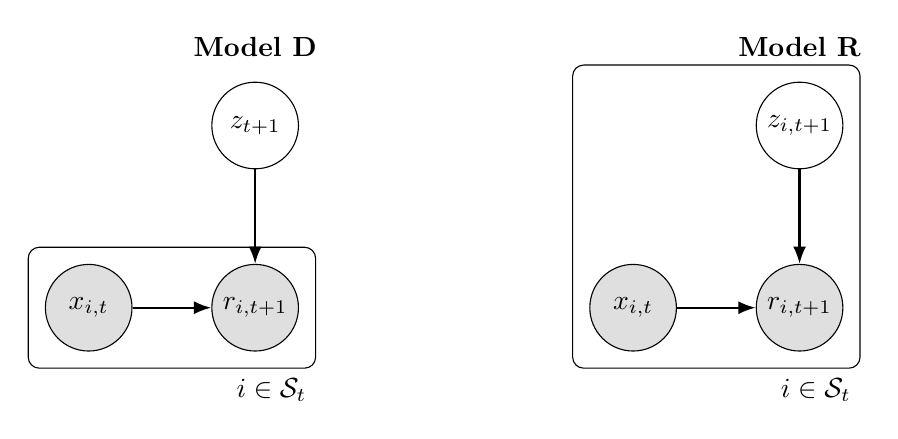
\begin{tikzpicture}[node distance=14mm]
\node[lat] (zD) {$z_{t+1}$};
\node[obs,below=12mm of zD] (rD) {$r_{i,t+1}$};
\node[obs,left=10mm of rD] (xD) {$x_{i,t}$};
\draw[edge] (zD)--(rD); \draw[edge] (xD)--(rD);
\begin{scope}[on background layer]
\node[plate,fit=(xD)(rD),label={[anchor=north east]south east:{$i\in\mathcal S_t$}}] {};
\end{scope}
\node[above=2mm of zD] {\textbf{Model D}};
\node[obs,right=58mm of rD] (rR) {$r_{i,t+1}$};
\node[lat,above=12mm of rR] (zR) {$z_{i,t+1}$};
\node[obs,left=10mm of rR] (xR) {$x_{i,t}$};
\draw[edge] (zR)--(rR); \draw[edge] (xR)--(rR);
\begin{scope}[on background layer]
\node[plate,fit=(xR)(rR)(zR),label={[anchor=north east]south east:{$i\in\mathcal S_t$}}] {};
\end{scope}
\node[above=2mm of zR] {\textbf{Model R}};
\end{tikzpicture}
\end{center}

\subsection*{D.2 The likelihood each model implies}

\paragraph{Model D.} Sum rule over the one latent of the date, then A3 (independence given the regime):
\begin{equation}
p_D\big(r_{\cdot,t+1}\big)=\sum_{k=1}^K\pi_k(t)\prod_{i\in\mathcal S_t}\N_{ik}
\quad\Rightarrow\quad
\ell_{\text{date}}(\theta)=\sum_t\log\sum_{k}\pi_k(t)\prod_{i}\N_{ik}.
\end{equation}

\paragraph{Model R.} Each stock has its own latent, so the sum over latents factorises stock by stock (the same step as Exercise A1(c)):
\begin{equation}
p_R\big(r_{\cdot,t+1}\big)=\prod_{i\in\mathcal S_t}\sum_{k=1}^K\pi_k(t)\,\N_{ik}
\quad\Rightarrow\quad
\ell_{\text{row}}(\theta)=\sum_t\sum_i\log\sum_k\pi_k(t)\,\N_{ik}.
\end{equation}
In D the sum sits outside the product; in R it sits inside.

\subsection*{D.3 The key identity: identical one-stock distributions}

\begin{keybox}{Proposition 1}
Under Model D, the distribution of one stock's return on its own is
\begin{equation*}
p_D\big(r_{i,t+1}\mid x_{\cdot,t},\F_t\big)=\sum_{k=1}^K\pi_k(t)\,\N_{ik},
\end{equation*}
which is exactly the factor of stock $i$ in Model R. The two models agree on every single stock and differ only in how stocks move \emph{together}.
\end{keybox}

\paragraph{Part 1: the independence used (d-separation).} In Model D the only path between $r_{i,t+1}$ and $r_{j,t+1}$ runs through $z_{t+1}$. Conditioning on $z_{t+1}$ blocks it (a tail-to-tail node), so given the regime the returns are independent. That is A3(a), read off the graph.

\paragraph{Part 2: the algebra.} Start from the joint of all returns and integrate out every stock except $i$:
\begin{equation*}
p_D(r_{i,t+1})=\int\sum_k\pi_k(t)\prod_{j}\N_{jk}\;\prod_{j\ne i}dr_{j,t+1}.
\end{equation*}
The sum over $k$ is finite, so it may be taken outside the integral:
\begin{equation*}
=\sum_k\pi_k(t)\,\N_{ik}\prod_{j\ne i}\int\N_{jk}\,dr_{j,t+1}.
\end{equation*}
Every remaining integral is the integral of a density, which is one:
\begin{equation*}
=\sum_k\pi_k(t)\,\N_{ik}.\qquad\blacksquare
\end{equation*}

\paragraph{Consequences.}
\begin{itemize}
  \item The point forecast $\sum_k\pi_k\mu_k$ and the whole one-stock predictive distribution are the same in both models.
  \item The models differ in the covariance between stocks. Writing $\mu_{ik}=\mu_k(x_{i,t})$, under D (Section 8.5),
  \begin{equation*}
  \Cov_D\big(r_{i,t+1},r_{j,t+1}\big)=\sum_k\pi_k(t)\big(\mu_{ik}-\bar\mu_i\big)\big(\mu_{jk}-\bar\mu_j\big),\qquad\bar\mu_i=\sum_k\pi_k\mu_{ik},
  \end{equation*}
  while under R it is zero. Stocks co-move under D because they share an unknown regime.
\end{itemize}

\subsection*{D.4 Composite likelihood}

\paragraph{Definition (Lindsay 1988).} Split the data into pieces $A_1,\dots,A_M$ (single observations, pairs, blocks) whose densities are known under the model. The composite log-likelihood is the weighted sum of the piece log-likelihoods:
\begin{equation*}
\ell_C(\theta)=\sum_{m=1}^M w_m\log p\big(y\in A_m;\theta\big).
\end{equation*}
It is a full likelihood only if the pieces happen to be independent. When each piece is one observation and the weights are one, $\ell_C$ is the \emph{independence likelihood}: the log-likelihood one would write if the observations were independent, evaluated with their correct marginals (Varin, Reid \& Firth 2011).

\paragraph{Application.} By Proposition 1, the correct marginal of stock-day $(i,t)$ under Model D is $\sum_k\pi_k\N_{ik}$. Hence
\begin{equation}
\ell_{\text{row}}(\theta)=\sum_t\sum_i\log p_D\big(r_{i,t+1};\theta\big)
\end{equation}
is the independence likelihood of Model D. The same function therefore has two readings: the exact likelihood of Model R, and a composite likelihood of Model D. Our study adopts the second reading. The model stays Model D; only the estimation objective changes.

\subsection*{D.5 Why it estimates the right parameters}

\paragraph{Step 1: each piece has an unbiased score.} Let $\theta_0$ be the true parameter and $p_i(r;\theta)$ the marginal density of piece $i$. Differentiating the identity that a density integrates to one,
\begin{equation*}
\int p_i(r;\theta)\,dr=1\quad\Rightarrow\quad\int\frac{\partial p_i(r;\theta)}{\partial\theta}\,dr=0\quad\Rightarrow\quad\E_{\theta_0}\Big[\frac{\partial}{\partial\theta}\log p_i(r;\theta)\Big|_{\theta_0}\Big]=0.
\end{equation*}
The last step writes the derivative of $p_i$ as $p_i$ times the derivative of $\log p_i$ and evaluates at $\theta_0$, where $p_i$ is the true density.

\paragraph{Step 2: a sum of unbiased scores is unbiased.} Expectation is linear, and it does not care whether the pieces are dependent:
\begin{equation*}
\E_{\theta_0}\big[\nabla\ell_{\text{row}}(\theta_0)\big]=\sum_t\sum_i\E_{\theta_0}\big[\nabla\log p_i(r_{i,t+1};\theta_0)\big]=0.
\end{equation*}
Dependence between the pieces would matter for the \emph{variance} of the sum, never for its mean.

\paragraph{Step 3: consistency.} The estimator solves $\nabla\ell_{\text{row}}(\hat\theta)=0$, an unbiased estimating equation. Under the usual regularity conditions it is consistent: as the number of dates grows, $\hat\theta\to\theta_0$. The conditions are a law of large numbers across dates and identifiability of $\theta$ from the one-stock marginals. Identifiability holds under mild conditions: the marginal is a finite Gaussian mixture of regressions, which is identified up to relabelling of the experts, and the frozen gate removes the relabelling by tying expert $k$ to HMM state $k$.

\subsection*{D.6 What it gives up: efficiency and standard errors}

Define the two matrices of estimating-equation theory:
\begin{equation*}
H(\theta_0)=-\E\big[\nabla^2\ell_{\text{row}}\big],\qquad J(\theta_0)=\Var\big[\nabla\ell_{\text{row}}\big].
\end{equation*}
For a full likelihood $H=J$, the Fisher information. For a composite likelihood they differ, because the pieces are dependent, and the asymptotic variance is the \emph{sandwich}
\begin{equation*}
\Var\big(\hat\theta\big)\approx H^{-1}JH^{-1}=G^{-1},\qquad G=HJ^{-1}H\ \text{(the Godambe information)}.
\end{equation*}
Two consequences:
\begin{itemize}
  \item \textbf{Efficiency.} $G$ is never larger than the Fisher information of the full likelihood. The information lost is exactly what the co-movement of stocks on a date says about the regime.
  \item \textbf{Standard errors.} The inverse Hessian alone, $H^{-1}$, is not a valid variance. Overlapping 5-day targets add dependence across dates, which works the same way.
\end{itemize}
Neither matters for the study, because inference comes from walk-forward rank ICs with Hansen--Hodrick corrections, never from the likelihood's curvature.

\subsection*{D.7 How the responsibilities behave}

Bayes' rule gives the posterior odds of regimes $k$ and $j$ after seeing the returns.

\paragraph{Per row:} one stock's evidence.
\begin{equation*}
\log\frac{\gamma_{i,t}(k)}{\gamma_{i,t}(j)}=\log\frac{\pi_k(t)}{\pi_j(t)}+\log\frac{\N_{ik}}{\N_{ij}}.
\end{equation*}

\paragraph{Per date:} the sum of all stocks' evidence.
\begin{equation*}
\log\frac{\gamma_t(k)}{\gamma_t(j)}=\log\frac{\pi_k(t)}{\pi_j(t)}+\sum_{i\in\mathcal S_t}\log\frac{\N_{ik}}{\N_{ij}}.
\end{equation*}

\paragraph{Size of the evidence.} If regime $k$ is true, each log-ratio term has expectation $\mathrm{KL}(\N_{\cdot k}\|\N_{\cdot j})>0$. With the example of Section 7.5 this is about $0.22$ nats per stock.
\begin{itemize}
  \item Per row the evidence is $0.22$ nats, a likelihood ratio of about $1.25$. The posterior stays close to the gate's prior.
  \item Per date it is about $0.22\times500=110$ nats. The posterior is $0$ or $1$ whatever the gate said.
\end{itemize}

\subsection*{D.8 When A3 is false}

\paragraph{A model in which A3 fails but the marginals are right.} Let stocks belong to clusters $c$ (industries) of size $m$, and add a shared cluster shock inside each regime:
\begin{equation*}
r_{i,t+1}=\mu_k(x_{i,t})+u_{c(i),t+1}+e_{i,t+1},\qquad u_c\sim\N(0,\rho s_k^2),\quad e_i\sim\N\big(0,(1-\rho)s_k^2\big),
\end{equation*}
independently. Two facts follow.
\begin{enumerate}
  \item \textbf{The one-stock marginal is unchanged.} The sum of two independent Gaussians is Gaussian with the variances added, $\rho s_k^2+(1-\rho)s_k^2=s_k^2$, so each stock is still $\sum_k\pi_k\N_{ik}$. The per-row objective is \emph{correctly specified}, and D.5 applies unchanged.
  \item \textbf{The joint is no longer a product.} Two stocks in the same cluster are correlated at $\rho$ within a regime. The per-date likelihood, which multiplies their densities, is \emph{misspecified}.
\end{enumerate}

\paragraph{How much evidence the per-date likelihood overcounts.} Write $v_i=\log(\N_{ik}/\N_{ij})$ for stock $i$'s evidence term in D.7, with variance $\sigma_v^2$, and let $\rho_v$ be the correlation of two such terms in the same cluster. It equals the return correlation $\rho$ when the two experts differ in their means, because $v_i$ is then linear in the return, and $\rho^2$ when they differ only in their noise levels, because $v_i$ is then linear in the squared residual. The variance of a sum of $N$ terms, in clusters of $m$ with correlation $\rho_v$ inside a cluster and zero across clusters, is
\begin{equation*}
\Var\Big(\sum_{i=1}^Nv_i\Big)=N\sigma_v^2\big(1+(m-1)\rho_v\big),
\end{equation*}
which is the variance of $N_{\text{eff}}$ independent terms, where
\begin{equation*}
N_{\text{eff}}=\frac{N}{1+(m-1)\rho_v}
\end{equation*}
(Kish's design effect). The per-date posterior treats the evidence as if it came from $N$ independent stocks, so it is overconfident by the factor $N/N_{\text{eff}}=1+(m-1)\rho_v$. With $m=45$ and $\rho_v=0.1$ the factor is $5.4$. In this illustration the values of $m$ and $\rho_v$ are assumed, not measured. In addition, the parameters that maximise a misspecified likelihood need not be $\theta_0$: they are the pseudo-true values that make the \emph{wrong joint} fit best. When the regimes are far apart this does little harm, because every date is still assigned correctly. When they are close, which is the realistic case for experts that differ by small corrections, overconfident misassignments feed back into the experts' means and noise levels.

\paragraph{A simulation check.} Simulate Model D with the cluster shock above: $K=2$, $T=600$ dates, $N=200$ stocks in clusters of $m=20$, gate weights drawn uniformly in $[0.1,0.9]$, and two close regimes with means $0$ and $0.05$ and noise levels $1$ and $1.08$. Then fit the means and noise levels by maximising each objective.
\begin{center}
\small\renewcommand{\arraystretch}{1.25}
\begin{tabular}{@{}lcccc@{}}
\toprule
 & $\mu_1$ & $\mu_2$ & $s_1$ & $s_2$ \\
\midrule
True values & $0$ & $0.05$ & $1$ & $1.08$ \\
A3 holds ($\rho=0$): per row & $-0.003$ & $0.050$ & $0.994$ & $1.088$ \\
A3 holds ($\rho=0$): per date & $-0.002$ & $0.049$ & $1.001$ & $1.082$ \\
A3 fails ($\rho=0.5$): per row & $-0.017$ & $0.070$ & $0.995$ & $1.079$ \\
A3 fails ($\rho=0.5$): per date & $-0.150$ & $0.230$ & $1.017$ & $1.023$ \\
\bottomrule
\end{tabular}
\end{center}
When A3 holds, both objectives recover the truth. When it fails, the per-row estimates stay close to it, while the per-date estimates are pulled away: the gap between the means is nearly eight times too large (0.38 against 0.05), and the noise levels are squeezed together. Even at the true parameters, the per-date posterior puts more than half its weight on the wrong regime on 14\% of dates when $\rho=0$ and on 35\% when $\rho=0.5$. This is one seed of a stylised example, not a measurement on the data.

\paragraph{The general principle.} An objective built from a lower-dimensional piece of the model (here, single stocks) needs only that piece to be right. This is the logic of generalised estimating equations with a working independence assumption (Liang \& Zeger 1986). The per-date likelihood needs the whole joint distribution to be right, and in a cross-section of 500 stocks it is not.

\subsection*{D.9 What this means for a frozen gate}

\begin{itemize}
  \item The gradient for expert $k$ on row $(i,t)$ is the regression residual weighted by the responsibility (Section 7.4). The responsibility therefore decides which data each expert learns from.
  \item \textbf{Per date:} $\gamma_t(k)\in\{0,1\}$ is set by the day's returns (D.7) and inflated by correlated evidence (D.8). Each expert learns from the days whose cross-section fits it, and the cross-section re-decides the regime every day. This is the daily version of the joint fit that Section 7.2 rules out, because it would let the stocks redefine the regimes.
  \item \textbf{Per row:} $\gamma_{i,t}(k)$ stays near $\pi_k(t)$. Each expert learns mainly from the days the gate assigns to its regime. The regimes remain \emph{market} regimes, which is why the gate was frozen (Q19).
  \item \textbf{The cost:} specialisation is softer, and the expert with the larger $s_k$ can attract outlying rows. Diagnostic: compare each expert's training weight with $\pi_k(t)$ and with the size of the residuals.
\end{itemize}

\subsection*{D.10 Summary}

\begin{center}
\small\renewcommand{\arraystretch}{1.3}
\begin{tabularx}{\textwidth}{@{}p{3.9cm}XX@{}}
\toprule
 & $\ell_{\text{date}}$ & $\ell_{\text{row}}$ (used) \\
\midrule
Status under Model D & exact likelihood & independence (composite) likelihood \\
One-stock distribution & $\sum_k\pi_k\N_{ik}$ & identical (Proposition 1) \\
Needs A3(a) & yes, the full joint & no, only the marginals \\
Consistent if A3 fails & not guaranteed; distorted when regimes are close (D.8) & yes (D.5, D.8) \\
Efficiency if the model is exactly right & full & lower (Godambe, D.6) \\
Standard errors from the Hessian & valid if A3 holds & invalid; sandwich needed \\
Responsibilities & $0$ or $1$, set by the returns & close to the gate's $\pi$ \\
Who defines the regime in training & the cross-section & the frozen gate \\
Mini-batches & whole dates & any rows \\
\bottomrule
\end{tabularx}
\end{center}

\emph{References:} Lindsay (1988), Contemporary Mathematics 80; Varin, Reid \& Firth (2011), Statistica Sinica 21; Liang \& Zeger (1986), Biometrika 73(1); Pakel, Shephard, Sheppard \& Engle (2021), JBES 39(3); Kish (1965), \emph{Survey Sampling}; Godambe (1960), Annals of Mathematical Statistics 31.


\end{document}
